\documentclass[12pt]{article}

% ── Packages ──────────────────────────────────────────────────────────────────
\usepackage[margin=2.5cm]{geometry}
\usepackage{lmodern}
\usepackage[T1]{fontenc}
\usepackage{amsmath,amssymb}
\usepackage{booktabs}
\usepackage{graphicx}
\usepackage{hyperref}
\usepackage[round]{natbib}
% \usepackage{multirow}   % unused
% \usepackage{array}      % unused
% \usepackage{tabularx}   % unused
\usepackage{float}
\usepackage{caption}
\usepackage{subcaption}
\usepackage{xcolor}
\usepackage{enumitem}
\usepackage{microtype}
\usepackage{tikz}
\usetikzlibrary{arrows.meta, positioning, calc}

\hypersetup{
  colorlinks=true,
  linkcolor=blue!60!black,
  citecolor=blue!60!black,
  urlcolor=blue!60!black
}

% ── Custom commands ───────────────────────────────────────────────────────────
\newcommand{\arcsinh}{\operatorname{arcsinh}}

\title{Beyond Price Levels: Foundation Model Embeddings Reveal\\a Hidden Dynamic Axis in Electricity Market Regimes}

\author{
  Carlo Mari \and
  Cristiano Baldassari\textsuperscript{*} \\[0.5em]
  \textit{Universit\`a degli Studi della Tuscia} \\
  Viterbo, Italy \\[0.3em]
  \textsuperscript{*}Corresponding author: \texttt{cristiano.baldassari@unitus.it}
}

\date{April 2026} %% TODO: aggiornare alla data di sottomissione

% ══════════════════════════════════════════════════════════════════════════════
\begin{document}
\maketitle

% ── Abstract ──────────────────────────────────────────────────────────────────
\begin{abstract}
Electricity market regimes are conventionally described along a single dimension, price level.
We demonstrate that this view misses an entire axis of market structure.
Using a fully non-parametric pipeline in which all parameters emerge from the data, we apply two representations to five years of ISO New England hourly prices and discover two statistically independent axes of regime organization.
An \emph{economic axis}, derived from hand-crafted price features, separates regimes by price level, from off-peak to extreme winter spike.
A \emph{dynamic axis}, derived from a time-series foundation model (MOMENT), separates regimes by temporal persistence, from fast mean-reversion to shock-persistent states.
The two axes are nearly orthogonal: knowing the price regime conveys almost no information about the dynamical mode, and vice versa.
This means that the conventional single-axis description systematically conflates market states that behave very differently: a high-price market that reverts quickly is operationally distinct from one that stays high for weeks, yet both receive the same ``spike'' label.
No single representation captures both dimensions; they must be deployed in parallel.

\medskip
\noindent\textbf{Keywords:} electricity spot markets, unsupervised regime detection, topological data analysis, time-series foundation models, diffusion maps
\end{abstract}

\newpage

% ══════════════════════════════════════════════════════════════════════════════
\section{Introduction}
\label{sec:introduction}

% --- 1.1 The economic context ---

Electricity is traded on wholesale markets where the price can change every hour.
Unlike oil, wheat, or other commodities, electricity cannot be stored in large quantities at reasonable cost: battery and pumped-hydro capacity covers only a small fraction of total demand.
As a result, supply must match demand at every instant, and the price reflects the cost of the last generator needed to keep the system in balance.

This generator, called the \emph{marginal generator}, is the most expensive unit currently dispatched.
In practice, generators are ranked by production cost (cheapest first) in a stack known as the \emph{merit order}.
When demand is low (nights, weekends, mild weather), cheap baseload generators (nuclear, large gas turbines) suffice, and prices are low.
When demand rises (heat waves, cold snaps) or supply drops (generator outages), the system must call on progressively more expensive units, gas peakers and in extreme cases oil-fired generators, and the price jumps accordingly.
This mechanism is the fundamental driver of regime formation \citep{weron2014}.

The resulting price series, called the Locational Marginal Price (LMP), exhibits statistical properties that set it apart from most financial assets: heavy tails (extreme price spikes), mean-reversion at multiple time scales, three overlapping seasonal cycles, a diurnal cycle (day/night demand), a weekly cycle (weekday/weekend), and an annual cycle (summer/winter heating and cooling demand), and occasional negative values when renewable generation exceeds demand \citep{ziel2018, weron2006}.
These regime shifts are driven by a confluence of factors (weather extremes, fuel-price shocks, renewable intermittency, transmission constraints, and generator outages) whose interactions produce the complex, non-stationary dynamics that make regime detection both important and difficult.

Identifying the prevailing market regime has direct practical consequences.
For market participants, regime-aware hedging strategies can reduce value-at-risk by conditioning portfolio adjustments on the current market state \citep{coulon2014}.
For system operators and regulators, persistent occupation of high-price regimes signals potential market-design deficiencies or the need for capacity-expansion interventions.
For forecasters, regime-switching models consistently outperform single-state benchmarks by allowing the conditional distribution of prices to adapt to the current operating environment \citep{janczura2013, nowotarski2018}.

% --- 1.2 Existing approaches and their limitations ---

Unsupervised regime detection in electricity markets remains an open methodological challenge.
The dominant paradigm relies on Hidden Markov Models (HMMs) or Gaussian Mixture Models (GMMs), which require the analyst to specify the number of states \emph{a priori} \citep{mount2006, kanamura2009}.
\citet{janczura2013} compared several HMM specifications and found that three-state models with heterogeneous variance provide the best fit for Nord Pool prices, but information criteria such as BIC or AIC, the standard tools for selecting the number of states, are known to be unreliable when the true data-generating process departs from the assumed parametric family, a near certainty with heavy-tailed electricity prices \citep{bierbrauer2007}.
More recent work has explored K-means and spectral clustering \citep{rintamaki2017}, yet these methods still depend on a pre-specified $K$ and struggle with non-convex cluster shapes, clusters that cannot be separated by hyperplanes, and density-varying geometries that arise in high-dimensional feature spaces.
As \citet{weron2014} noted in a comprehensive survey, regime identification remains ``one of the most challenging problems in the field.''

% --- 1.3 The multi-dimensional nature of regimes ---

A key limitation of existing approaches is that they describe the market state with a single label.
Yet a market regime has at least two distinct dimensions.
The first is \emph{price level}: how expensive is electricity right now, off-peak, normal, or spike?
The second is \emph{price dynamics}: how does the price behave over time, does it revert quickly to its normal level after a shock, or does the shock persist for days?
These two dimensions carry different information.
A market at \$100/MWh that will revert to \$50 within hours poses a different risk than a market at \$100/MWh that will stay elevated for two weeks, yet a single regime label (``spike'') conflates the two.
Existing regime-switching models \citep{huisman2003} assign a single latent state that simultaneously governs both the price level and the volatility dynamics, implicitly assuming that the two dimensions are driven by the same process.
Whether this assumption holds, whether level and dynamics are indeed coupled or instead vary independently, is an empirical question that has not been tested.

% --- 1.4 New tools ---

Two recent developments create an opportunity to test it.
First, \emph{time-series foundation models}, large neural networks pre-trained on diverse time series, can produce embeddings that summarize the temporal structure of an input window without domain-specific training \citep{yeh2023}.
Second, topological data analysis offers clustering methods that determine the number of regimes directly from the data, without requiring the analyst to specify $K$ in advance.
Neither tool has been applied to electricity-market regime detection.

% --- 1.4 Research question ---

Together, these tools make it possible to test whether level and dynamics are governed by the same latent structure or by independent processes.
The strategy is to construct two representations of the same price data, one that encodes price-level information through domain-specific statistics and one that encodes temporal dynamics through a foundation model, and to cluster each independently with the same non-parametric algorithm.
If the two partitions agree, level and dynamics are coupled and the market's regime structure is one-dimensional.
If they disagree, the two dimensions vary independently, and a single regime label is insufficient.

% --- 1.5 Contribution ---

This paper provides an answer.
We construct a fully non-parametric pipeline (Figure~\ref{fig:pipeline}) in which the number of regimes and all algorithmic parameters emerge from the data rather than the analyst's choice.
Crucially, the pipeline clusters on deseasonalized residuals, not on raw prices: the absolute price level is removed before clustering and used only afterwards, as an external variable, to characterize and validate the resulting regimes.
Applying this pipeline to five years of ISO New England hourly LMPs with two representations, one encoding price-level features and the other encoding temporal dynamics via a foundation model, we find that the two resulting partitions are statistically independent: the electricity market is organized along at least two orthogonal axes of regime structure, one economic and one dynamic, each capturing a dimension of market variation invisible to the other.
% ── Pipeline diagram ─────────────────────────────────────────────────────────
\begin{figure}[H]
\centering
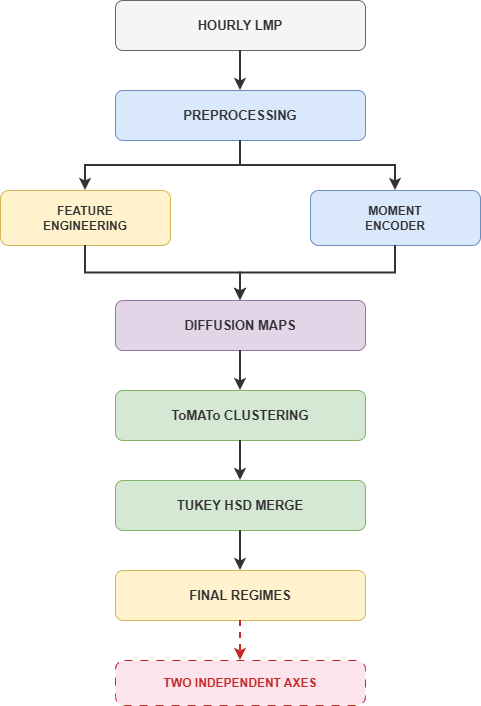
\includegraphics[width=0.65\textwidth]{pipeline_v9.drawio.png}
\caption{Non-parametric regime-detection pipeline.}
\label{fig:pipeline}
\end{figure}

The complete pipeline code and data-processing scripts are publicly available at \url{https://github.com/TODO/nepool-tda}. %% TODO: inserire URL reale

The remainder of the paper is organized as follows.
Section~\ref{sec:methodology} describes the data and the pipeline.
Section~\ref{sec:results} presents the empirical results.
Section~\ref{sec:discussion} discusses implications and limitations.
Section~\ref{sec:conclusion} concludes.


% ══════════════════════════════════════════════════════════════════════════════
\section{Data and Methodology}
\label{sec:methodology}

The pipeline consists of four stages: data acquisition and preprocessing, representation extraction, dimensionality reduction via Diffusion Maps, and clustering with post-hoc merging (see Figure~\ref{fig:pipeline}).

% ── 2.1 Data and Preprocessing ──────────────────────────────────────────────
\subsection{Data and Preprocessing}
\label{sec:preprocessing}

Hourly day-ahead LMPs for the ISO New England Massachusetts Hub are downloaded from the U.S.\ Energy Information Administration (EIA).\footnote{EIA Open Data API v2: \url{https://api.eia.gov/v2/electricity/rto/wholesale-data}. Query parameters: \texttt{respondent=ISNE}, \texttt{type=D} (day-ahead). A free API key is required, obtainable at \url{https://www.eia.gov/opendata/register.php}. Hourly LMPs are returned in JSON; we convert to a single Parquet file covering 2021--2025.}
The Locational Marginal Price (LMP) is the wholesale price of electricity at a specific node of the transmission grid, determined hourly through a competitive auction in which generators submit supply offers and the system operator clears the market.
The Massachusetts Hub is a reference pricing node widely used as a benchmark for the New England region.

The sample contains 43,814 hourly observations spanning January 2021 through December 2025 (Table~\ref{tab:lmp_stats}).
This five-year window captures several distinct market episodes: the post-COVID demand recovery (2021), the natural-gas price spike driven by the Russia--Ukraine conflict (2022), the subsequent normalization (2023--2024), and several extreme winter cold events that triggered price spikes exceeding \$400/MWh.

\begin{table}[H]
\centering
\caption{Descriptive statistics of ISONE Massachusetts Hub LMP (\$/MWh), 2021--2025.}
\label{tab:lmp_stats}
\begin{tabular}{lccccc}
\toprule
& $n$ & Mean & Std & Skewness & Kurtosis \\
\midrule
LMP (\$/MWh) & 43,814 & 55.51 & 42.37 & 2.34 & 9.94 \\
\bottomrule
\end{tabular}
\end{table}

Electricity prices span a wide range (from near-zero to over \$400/MWh in our sample) and can take negative values during periods of renewable oversupply.
To stabilize the variance while preserving the full support of the distribution, we apply the area-hyperbolic-sine transformation,
\begin{equation}
y_t = \arcsinh(p_t) = \ln\!\left(p_t + \sqrt{p_t^2 + 1}\right),
\label{eq:arcsinh}
\end{equation}
which is defined on all of $\mathbb{R}$, requires no tuning parameters, and has a useful dual behavior: for large $|p|$ it acts like $\log(2|p|)$, compressing extreme spikes; near zero it is approximately linear, preserving the fine structure of normal-regime price movements.

The transformed series $y_t$ carries strong seasonality at three scales: 24\,h (day/night demand cycle), 168\,h (weekday/weekend pattern), and 8,760\,h (annual summer/winter cycle).
If not removed, these seasonal components dominate the clustering, which would merely rediscover ``summer versus winter'' rather than structural market regimes.
We apply MSTL (Multi-Seasonal-Trend decomposition using Loess) \citep{bandara2021}, a generalization of STL \citep{cleveland1990} that handles multiple seasonal periods simultaneously.
STL decomposes a time series into trend, one seasonal component, and residual using locally weighted regression (Loess); MSTL extends this to an arbitrary number of seasonal periods by iteratively extracting each cycle:
\begin{equation}
y_t = \tau_t + s_t^{(24)} + s_t^{(168)} + s_t^{(8760)} + r_t,
\label{eq:mstl}
\end{equation}
where $\tau_t$ is the trend, $s_t^{(P)}$ are the seasonal components at period $P$, and $r_t$ is the residual, the deseasonalized signal that serves as input to regime detection.
Figure~\ref{fig:mstl} shows all five components.

\begin{table}[H]
\centering
\caption{Descriptive statistics of the MSTL residual $r_t$.}
\label{tab:residual_stats}
\begin{tabular}{lcccc}
\toprule
& Mean & Std & Skewness & Kurtosis \\
\midrule
MSTL residual $r_t$ & 0.003 & 0.298 & 0.34 & 4.38 \\
\bottomrule
\end{tabular}
\end{table}

\noindent The residual has substantially lighter tails than the raw LMP (kurtosis 4.38 vs.\ 9.94), confirming that the arcsinh transformation and seasonal removal have absorbed most of the extreme variation.

\begin{figure}[H]
\centering
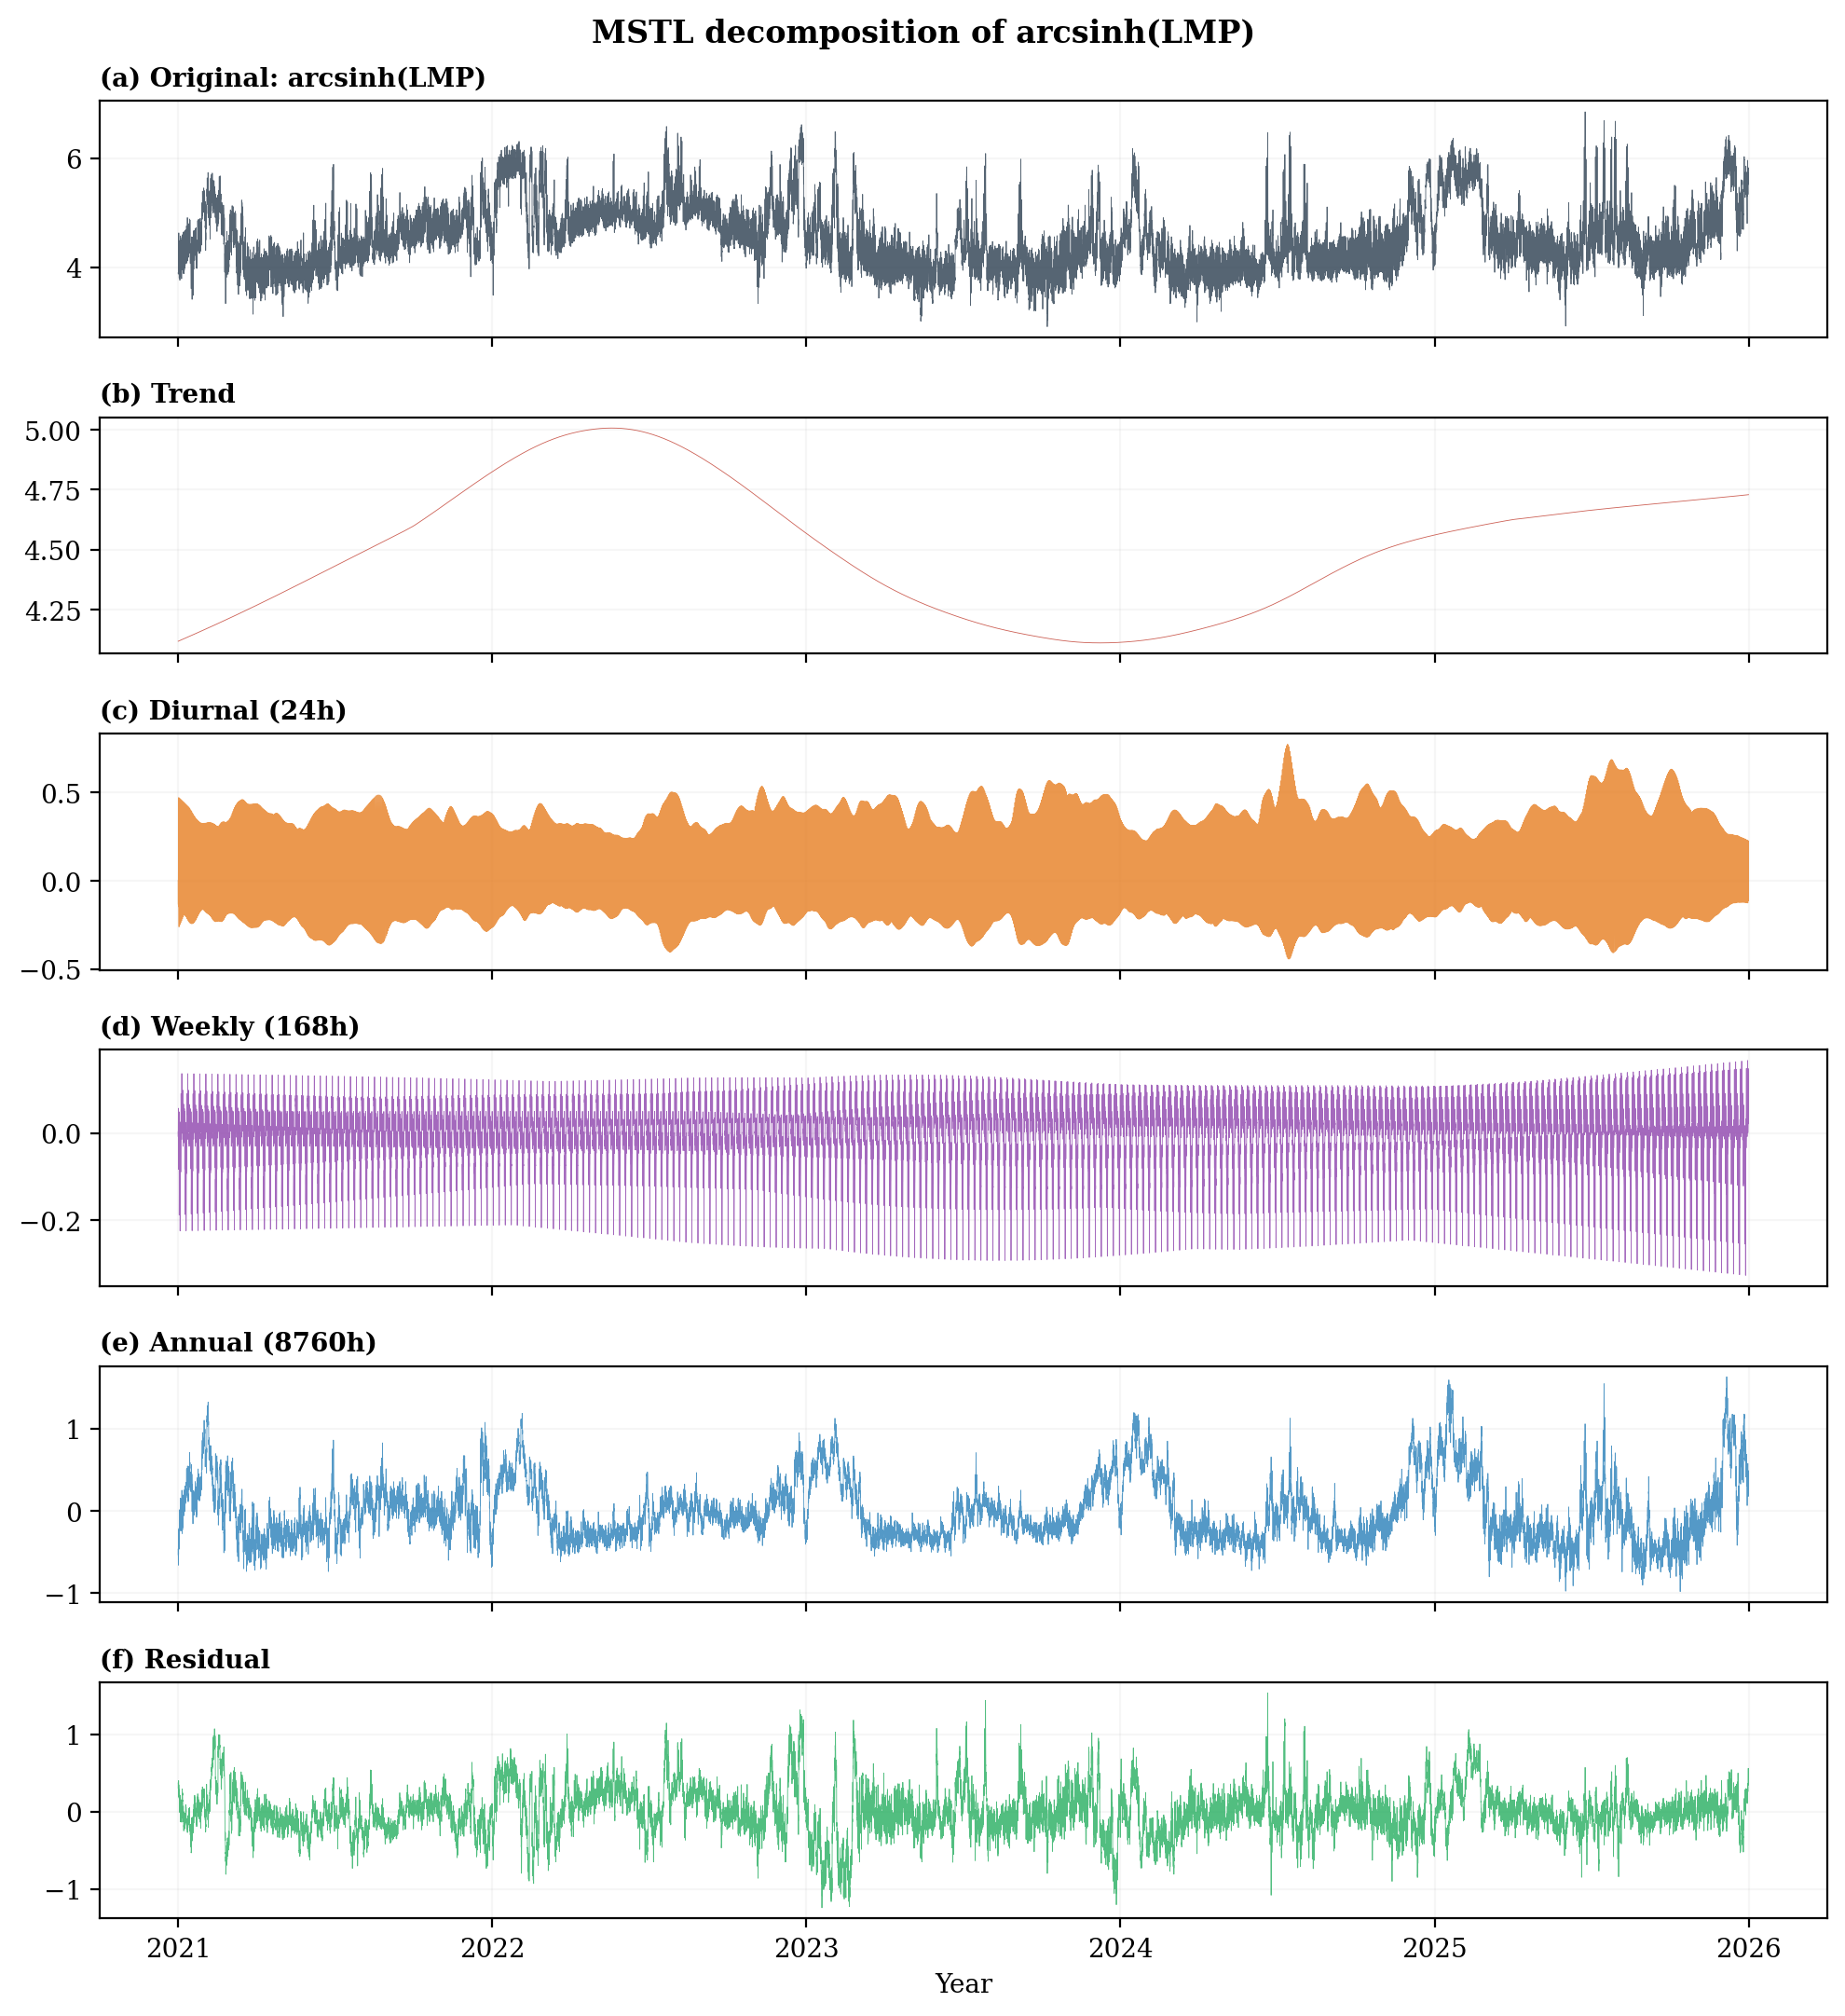
\includegraphics[width=0.75\textwidth]{mstl_decomposition.png}
\caption{MSTL decomposition of arcsinh(LMP). (a) original series; (b) trend; (c) diurnal seasonal; (d) weekly seasonal; (e) annual seasonal; (f) residual.}
\label{fig:mstl}
\end{figure}

To verify effective deseasonalization we examine the autocorrelation function (ACF).
The ACF at lag $h$, denoted $\rho(h)$, measures the linear correlation between $y_t$ and $y_{t+h}$: a value near 1 indicates that the series repeats itself $h$ steps later, while a value near 0 indicates no such repetition.
Table~\ref{tab:acf} shows that the lag-24 ACF drops from 0.890 to 0.012 after MSTL decomposition, and the lag-168 ACF drops from 0.678 to 0.003, confirming that the diurnal and weekly cycles have been effectively removed.
Crucially, the residual retains strong hourly persistence (lag-1 ACF $= 0.851$): the seasonal structure is removed but the serial dependence that distinguishes different market dynamics is preserved.

\begin{table}[H]
\centering
\caption{Autocorrelation before and after MSTL decomposition.}
\label{tab:acf}
\begin{tabular}{lcccc}
\toprule
& Lag 1 & Lag 24 & Lag 168 & Lag 8760 \\
\midrule
arcsinh(LMP)     & 0.963 & 0.890 & 0.678 & 0.108 \\
MSTL residual    & 0.851 & 0.012 & 0.003 & 0.001 \\
\bottomrule
\end{tabular}
\end{table}

MSTL is applied globally to the full 43,814-hour series before any windowing.
At this point, we have a single long sequence of hourly residuals $r_1, r_2, \ldots, r_{43814}$.
The next step converts this sequence into a collection of shorter episodes that can be compared, represented, and clustered.

A single residual value $r_t$ describes the market at one hour, but a market regime is a sustained state that lasts for days or weeks.
Detecting regimes therefore requires examining blocks of consecutive hours rather than individual observations: is the price stable or volatile over this period? Does it revert quickly after a shock, or does the shock persist?

Each such block is called a \emph{window}: a contiguous segment of $W$ consecutive hourly residual values.
We set $W = 512$ hours, approximately 21 days, so that each window spans at least three full weekly cycles and captures enough temporal structure for the downstream representations to work with.
Windows are placed along the time axis with a stride of $S = 6$ hours: a new window starts every 6 hours.
Consecutive windows therefore overlap heavily --- they share $W - S = 506$ of their 512 hours --- but the 6-hour offset provides four snapshots per day, giving sufficient temporal resolution to track regime transitions.
The calibration of $W$ and $S$ is discussed in Section~\ref{sec:calibration}.
With these parameters, the full series yields $N = 7{,}217$ windows.

Each window is timestamped at its final hour.
Let $t_1$ be the final hour of the first window.
The final hour of window $i$ is
\begin{equation}
t_i = t_1 + (i-1)\,S,
\qquad
i=1,\ldots,N.
\label{eq:window_count}
\end{equation}
Window $i$ then collects the $W = 512$ residual values ending at hour $t_i$:
\begin{equation}
\mathbf{r}_i =
\bigl(r_{t_i-511},\;\, r_{t_i-510},\;\, \ldots,\;\, r_{t_i}\bigr).
\label{eq:window_vectors}
\end{equation}
For FE features that require raw prices (Section~\ref{sec:repr_fe}), we also retain the corresponding raw-price window $\mathbf{p}_i = (p_{t_i-511}, \ldots, p_{t_i})$.
To make this concrete: the first window $\mathbf{r}_1$ covers hours $t_1 - 511$ through $t_1$; the second window $\mathbf{r}_2$ starts 6 hours later and covers hours $t_1 - 505$ through $t_1 + 6$.
The two windows share 506 of their 512 hours and differ only in the 6 oldest and 6 newest observations (Figure~\ref{fig:windows}).

From this point onward, each window is one observation: it receives one representation vector, one cluster label, and one regime assignment.
All subsequent analysis is indexed by $i = 1, \ldots, 7{,}217$.

\begin{figure}[H]
\centering
\resizebox{0.92\textwidth}{!}{%
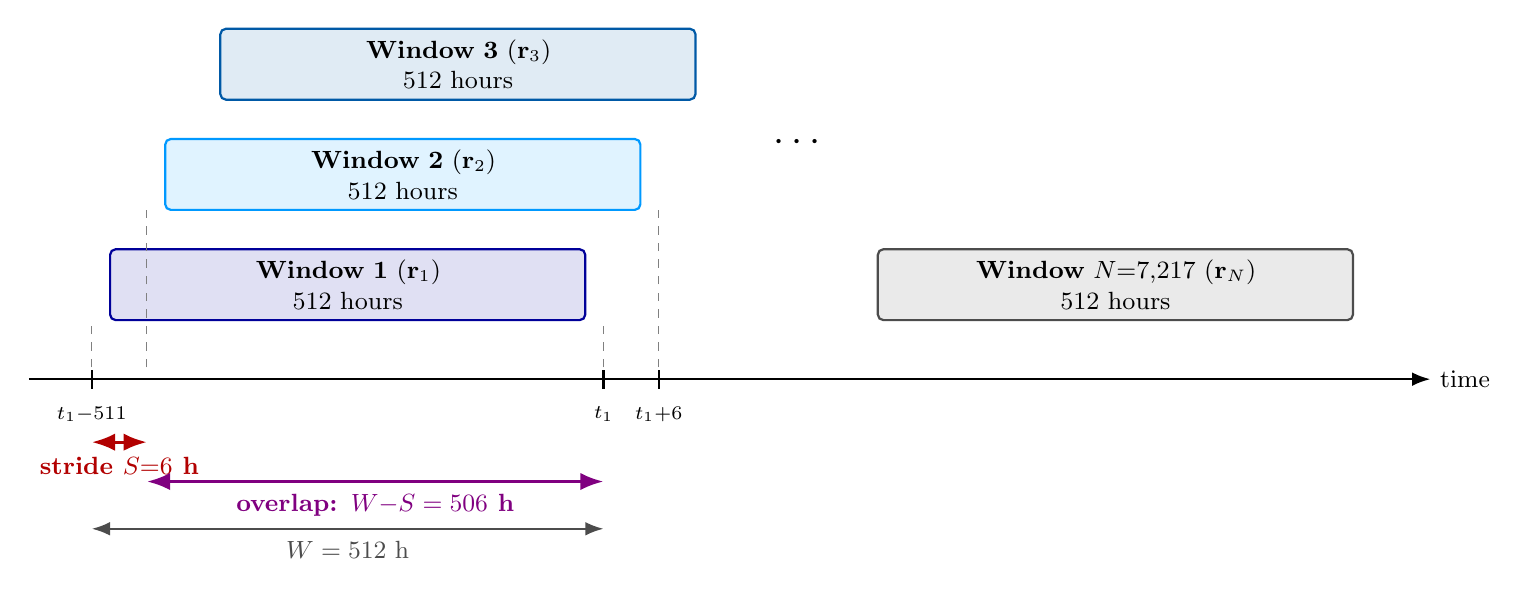
\begin{tikzpicture}[
  font=\small,
  >=Latex,
  win/.style={draw=#1, fill=#1!12, thick, rounded corners=2pt, minimum height=0.9cm}
]

% Time axis
\draw[->, thick] (-0.3,0) -- (17.5,0);
\node[font=\small, right] at (17.5, 0) {time};

% Tick marks on time axis — only window 1 boundaries
\draw[thick] (0.5, -0.12) -- (0.5, 0.12);
\node[font=\scriptsize, below=3pt] at (0.5, -0.12) {$t_1{-}511$};
\draw[thick] (7, -0.12) -- (7, 0.12);
\node[font=\scriptsize, below=3pt] at (7, -0.12) {$t_1$};
\draw[thick] (7.7, -0.12) -- (7.7, 0.12);
\node[font=\scriptsize, below=3pt] at (7.7, -0.12) {$t_1{+}6$};

% Window 1 — bottom row
\node[win=blue!60!black, text width=5.8cm, align=center] (w1) at (3.75, 1.2)
  {\textbf{Window 1} ($\mathbf{r}_1$)\\ 512 hours};

% Window 2 — shifted right by stride, slightly above
\node[win=blue!40!cyan, text width=5.8cm, align=center] (w2) at (4.45, 2.6)
  {\textbf{Window 2} ($\mathbf{r}_2$)\\ 512 hours};

% Window 3 — shifted again
\node[win=blue!30!teal, text width=5.8cm, align=center] (w3) at (5.15, 4.0)
  {\textbf{Window 3} ($\mathbf{r}_3$)\\ 512 hours};

% Dots
\node[font=\Large] at (9.5, 3.0) {$\cdots$};

% Window N
\node[win=gray!60!black, text width=5.8cm, align=center] (wN) at (13.5, 1.2)
  {\textbf{Window $N{=}7{,}217$} ($\mathbf{r}_N$)\\ 512 hours};

% Dashed lines from window edges to time axis
\draw[dashed, gray, thin] (0.5, 0.15) -- (0.5, 0.75);
\draw[dashed, gray, thin] (7.0, 0.15) -- (7.0, 0.75);
\draw[dashed, gray, thin] (1.2, 0.15) -- (1.2, 2.15);
\draw[dashed, gray, thin] (7.7, 0.15) -- (7.7, 2.15);

% Stride annotation
\draw[<->, very thick, red!70!black] (0.5, -0.8) -- (1.2, -0.8);
\node[font=\small\bfseries, red!70!black, below=2pt] at (0.85, -0.8) {stride $S{=}6$ h};

% Overlap annotation — large bracket under windows
\draw[<->, very thick, violet] (1.2, -1.3) -- (7.0, -1.3);
\node[font=\small\bfseries, violet, below=1pt] at (4.1, -1.3) {overlap: $W{-}S = 506$ h};

% Window width annotation
\draw[<->, thick, black!70] (0.5, -1.9) -- (7.0, -1.9);
\node[font=\small, black!70, below=1pt] at (3.75, -1.9) {$W = 512$ h};

\end{tikzpicture}%
}
\caption{Sliding-window scheme. Each window contains $W=512$ consecutive hourly residuals. Consecutive windows start $S=6$ hours apart and overlap by $W-S = 506$ hours. The same scheme produces $N = 7{,}217$ windows from the full series.}
\label{fig:windows}
\end{figure}

\noindent This notation is useful because every subsequent object in the analysis is attached to the same index $i$: the FE features, the MOMENT embedding, and the final regime labels all describe the same 512-hour market episode.

% ── 2.2 Representations ──────────────────────────────────────────────────────
\subsection{Representations}
\label{sec:representations}

Clustering algorithms cannot operate directly on raw time-series windows of 512 values: the space is too high-dimensional, and the signal-to-noise ratio is poor.
Each window must first be compressed into a lower-dimensional vector, a \emph{representation}, that preserves the information relevant to regime structure while discarding noise.

To test whether a single partition suffices to describe the market's regime structure, we construct two representations that encode the data from fundamentally different perspectives.
The first is a set of domain-specific features designed to capture known properties of electricity prices.
The second is a domain-agnostic foundation model that receives the raw residual series and encodes whatever structure it finds, with no assumptions about electricity markets.
For each window $i$, the two representations can be written compactly as
\begin{equation}
\mathbf{x}_i^\text{FE} = \Phi_\text{FE}(\mathbf{r}_i,\mathbf{p}_i) \in \mathbb{R}^{19},
\qquad
\mathbf{x}_i^\text{MOM} = \Phi_\text{MOM}(\mathbf{r}_i) \in \mathbb{R}^{1024}.
\label{eq:representations}
\end{equation}
If the two representations produce the same partition, a single axis suffices; if they diverge, the market has at least two independent dimensions of regime structure, and the divergence is genuine, because the foundation model has no prior knowledge of price levels.

\subsubsection{Feature Engineering}
\label{sec:repr_fe}

The first representation uses feature engineering, the manual design of numerical summaries that capture known properties of the data.
For each 512-hour window, we compute 19 features (reported in Table~\ref{tab:features}) that encode domain knowledge about electricity prices, following the feature taxonomy used in electricity-price regime analysis \citep{escribano2011, knittel2005}.
The features are organized into four groups:
(i) distributional statistics (11 features) characterize the shape of the price distribution within each window (mean, standard deviation, skewness, kurtosis, minimum, maximum, range, median, 5th and 95th percentiles, and interquartile range), capturing whether the window contains mostly stable prices or is prone to extreme events, computed on the MSTL residual to focus on regime-related variation rather than seasonal patterns;
(ii) temporal persistence (4 features) measures the autocorrelation function (ACF) at lags of 1, 6, 24, and 168 hours, where the ACF at lag $h$ is the correlation between $r_t$ and $r_{t+h}$, encoding how quickly the market reverts to equilibrium after a shock;
(iii) intra-day volatility (1 feature) measures the average absolute hourly price change within 24-hour blocks;
(iv) raw LMP statistics (3 features) are computed on the untransformed LMP in \$/MWh (mean, 95th percentile, standard deviation), retaining the absolute price level that the arcsinh transformation and MSTL decomposition remove.

\begin{table}[H]
\centering
\caption{Hand-crafted features.}
\label{tab:features}
\footnotesize
\setlength{\tabcolsep}{3pt}
\begin{tabular}{rllp{4.2cm}}
\toprule
\# & Feature & Computed on & Captures \\
\midrule
\multicolumn{4}{l}{\textit{Distributional statistics (11 features, on MSTL residual)}} \\
1  & Mean             & $\bar{r}_w$ & Deseasonalized price level \\
2  & Std              & $\sigma_{r,w}$ & Volatility \\
3  & Skewness         & $\gamma_1(r_w)$ & Asymmetry (positive = spike-prone) \\
4  & Kurtosis         & $\gamma_2(r_w)$ & Tail heaviness \\
5  & Minimum          & $\min(r_w)$ & Deepest trough in window \\
6  & Maximum          & $\max(r_w)$ & Spike magnitude \\
7  & Range            & $\max - \min$ & Total excursion \\
8  & Median           & $Q_{50}(r_w)$ & Robust center \\
9  & 5th percentile   & $Q_{5}(r_w)$ & Lower tail \\
10 & 95th percentile  & $Q_{95}(r_w)$ & Upper tail \\
11 & IQR              & $Q_{75} - Q_{25}$ & Robust dispersion \\
\midrule
\multicolumn{4}{l}{\textit{Temporal persistence (4 features, on MSTL residual)}} \\
12 & ACF lag 1\,h     & $\hat{\rho}_1(r_w)$ & Hour-to-hour persistence \\
13 & ACF lag 6\,h     & $\hat{\rho}_6(r_w)$ & Intra-day persistence \\
14 & ACF lag 24\,h    & $\hat{\rho}_{24}(r_w)$ & Residual diurnal pattern \\
15 & ACF lag 168\,h   & $\hat{\rho}_{168}(r_w)$ & Residual weekly pattern \\
\midrule
\multicolumn{4}{l}{\textit{Intra-day volatility (1 feature, on MSTL residual)}} \\
16 & vol\_24h         & Mean $|\Delta r|$ per 24\,h block & Average intra-day price movement \\
\midrule
\multicolumn{4}{l}{\textit{Raw price statistics (3 features, on untransformed LMP in \$/MWh)}} \\
17 & LMP mean         & $\bar{p}_w$ & Absolute price level \\
18 & LMP 95th pct     & $Q_{95}(p_w)$ & Absolute spike level \\
19 & LMP std          & $\sigma_{p,w}$ & Absolute volatility \\
\bottomrule
\end{tabular}
\end{table}

All 19 features are standardized to zero mean and unit variance before subsequent analysis, so that variables measured in different units (ACF, residual volatility, LMP in \$/MWh) are placed on a comparable scale.
No explicit feature selection or weighting is performed: we retain all 19 features and let the downstream dimensionality reduction determine which dimensions contribute most to the manifold geometry.
Note that FE includes 4 temporal-persistence features (ACF at lags 1, 6, 24, 168\,h), but these are only 4 out of 19 dimensions (21\%); the remaining 15 distributional and price-level features are expected to dominate the manifold geometry.
This motivates a second, complementary representation that approaches the data without domain assumptions.

\subsubsection{MOMENT Foundation Model}
\label{sec:repr_moment}

The second representation is produced by MOMENT-1-large\footnote{\url{https://github.com/moment-timeseries-foundation-model/moment}} \citep{moment2024}, a transformer-based time-series foundation model with 340 million parameters.
Unlike the hand-crafted features, MOMENT receives the raw 512-hour residual window as input and produces a 1,024-dimensional embedding vector through its encoder, without any training or fine-tuning on electricity data: the model is applied exactly as pre-trained (zero-shot inference).

MOMENT is pre-trained on a large corpus of over 385,000 time series from diverse domains such as weather, finance, healthcare, and engineering (the Time-Series Pile\footnote{\url{https://huggingface.co/datasets/AutonLab/Timeseries-PILE}}).
During pre-training, random portions of the input are hidden and the model learns to fill in the gaps from the surrounding context.
To succeed, the model must learn how temporal patterns develop over time, which is precisely the kind of information we want it to encode.
We choose MOMENT over alternative foundation models (Chronos \citep{chronos2024}, TimesFM \citep{timesfm2024}, Moirai \citep{woo2024}) because it is the only open model that provides a native embedding mode designed for representation learning, rather than only forecasting.

The resulting 1,024-dimensional embedding is domain-agnostic: it knows nothing about electricity prices, merit order, or market structure.
Any structure it captures is therefore learned purely from the temporal dynamics of the residual series.

% ── 2.3 Dimensionality Reduction ─────────────────────────────────────────────
\subsection{Dimensionality Reduction via Diffusion Maps}
\label{sec:diffmaps}

Each sliding window is now represented as a vector: 19 numbers for the FE representation, or 1,024 numbers for MOMENT.
Clustering directly in these high-dimensional spaces poses two problems.
First, distances between points become increasingly uniform as dimensionality grows --- a phenomenon known as the \emph{curse of dimensionality} \citep{beyer1999} --- which makes it difficult for clustering algorithms to distinguish nearby points from distant ones.
Second, the data may not fill the full ambient space.
Instead, the windows may lie on a curved, lower-dimensional surface (a \emph{manifold}), so that the straight-line Euclidean distance between two points is a poor measure of their true proximity along the data surface.
Dimensionality reduction addresses both problems by finding a small number of coordinates that faithfully represent the geometry of the data.

We use Diffusion Maps \citep{coifman2006}, a nonlinear method specifically designed for manifold data.
The steps below are applied independently to each representation: once to the 19-dimensional FE vectors and once to the 1,024-dimensional MOMENT embeddings.
The algorithm is the same in both cases, but the input, the selected number of coordinates, and the resulting geometry may differ.

The first step builds a weighted graph over the $N = 7{,}217$ windows.
Let $\mathbf{x}_i$ denote the representation vector of window $i$ (either FE or MOMENT).
For every pair of windows $i$ and $j$, Diffusion Maps computes an affinity score:
\begin{equation}
w_{ij}
=
\exp\!\left(
-\frac{\|\mathbf{x}_i-\mathbf{x}_j\|^2}{\epsilon}
\right).
\label{eq:diffusion_kernel}
\end{equation}
The Gaussian kernel assigns large weights to pairs of windows whose representation vectors are close and weights near zero to pairs that are far apart.
The bandwidth $\epsilon$ controls the scale: a small $\epsilon$ makes only very close neighbors count, while a large $\epsilon$ blurs the structure.
We set $\epsilon$ to the median of all pairwise squared distances, a common data-driven default that adapts to the natural spread of the representation.

The second step converts the affinities into transition probabilities.
Each row of the affinity matrix is normalized to sum to 1:
\begin{equation}
P_{ij} =
\frac{w_{ij}}{\sum_{\ell=1}^{N} w_{i\ell}}.
\label{eq:diffusion_transition}
\end{equation}
The result is a transition matrix that can be interpreted as a random walk on the data graph: $P_{ij}$ is the probability that a walker sitting on window $i$ moves to window $j$ in one step.
Windows in dense regions are connected to many high-weight neighbors, so walkers move easily within them.
Windows in sparse regions are reached only by long, low-probability paths.
This random-walk perspective is the key advantage of Diffusion Maps over linear methods like PCA: it measures proximity \emph{along the data manifold} rather than through empty space.

The third step extracts low-dimensional coordinates from the transition matrix.
The leading eigenvectors of $P$ capture the dominant directions along which the random walk spreads.
Let $\psi_1,\ldots,\psi_d$ be the first $d$ non-trivial eigenvectors, sorted by decreasing eigenvalue $\lambda_1 \geq \cdots \geq \lambda_d$.
The diffusion coordinates of window $i$ are
\begin{equation}
\Psi_d(i)
=
\bigl(\lambda_1 \psi_1(i),\ldots,\lambda_d \psi_d(i)\bigr).
\label{eq:diffusion_coordinates}
\end{equation}
Each eigenvalue $\lambda_k$ reflects the importance of the corresponding direction: large eigenvalues capture dominant geometric structures (broad separations in the data), while small eigenvalues capture fine-scale noise.
Multiplying each eigenvector by its eigenvalue ensures that the coordinates are scaled by relevance.
The result is a $d$-dimensional vector for each window that preserves the neighborhood structure of the original high-dimensional representation.

The number of diffusion coordinates $d$ must be chosen.
We sweep over $d \in \{2, 3, \ldots, 20\}$ and for each candidate compute the diffusion coordinates, run a preliminary clustering, and evaluate the silhouette score \citep{rousseeuw1987}.
The silhouette score measures how well each point fits its assigned cluster compared to the next-best alternative; it depends only on the geometry of the diffusion space, not on any economic variable.
We retain the $d$ that maximizes this score.
The selected dimensionalities are reported in Table~\ref{tab:dimred}: 11 coordinates for FE and 2 for MOMENT.
The fact that MOMENT collapses to just 2 dimensions is itself informative: it suggests that the foundation model's representation is organized along a small number of dominant temporal modes.

\begin{table}[H]
\centering
\caption{Dimensionality reduction via Diffusion Maps.}
\label{tab:dimred}
\small
\begin{tabular}{lcc}
\toprule
Representation & Input dimensions & After Diffusion Maps \\
\midrule
FE     & 19    & 11 \\
MOMENT & 1,024 & 2 \\
\bottomrule
\end{tabular}
\end{table}


% ── 2.4 Clustering ────────────────────────────────────────────────────────────
\subsection{Clustering via ToMATo and Tukey HSD Merge}
\label{sec:clustering}

The next step partitions the diffusion coordinates into discrete regimes.
The procedure has two stages: first, a topological algorithm discovers an intentionally fine-grained set of density modes; then, a statistical test consolidates modes that are indistinguishable on the relevant market variable.

\paragraph{Stage 1: mode discovery via ToMATo.}
We use ToMATo (Topological Mode Analysis Tool) \citep{chazal2013}, a clustering algorithm from topological data analysis that makes no assumption about cluster shape and does not require the number of clusters $K$ to be specified in advance.

ToMATo works by building a density landscape over the diffusion space and identifying its peaks.
The first step is to estimate how dense the data is around each point, using the log-distance-to-a-measure (logDTM) \citep{chazal2011dtm}.
Intuitively, if a point's $k$ nearest neighbors are all close by, the point lies in a crowded region (low score); if the neighbors are far away, the point is isolated (high score).
Formally, for a diffusion point $\Psi_d(i)$:
\begin{equation}
\ell_i
=
\log\!\left[
\left(
\frac{1}{k}
\sum_{q=1}^{k}
\|\Psi_d(i)-\Psi_d(i_q)\|^2
\right)^{1/2}
\right],
\label{eq:logdtm}
\end{equation}
where $i_1,\ldots,i_k$ are the $k$ nearest neighbors.
The parameter $k$ controls the smoothness of the density estimate and is selected by grid search over $k \in \{20, 40, 60, 80, 100, 150\}$.

The second step is to find the peaks of this density landscape and decide which ones are real.
ToMATo sweeps a threshold from high density to low density.
As the threshold descends, density peaks appear (\emph{birth}); as it continues, smaller peaks merge into taller neighbors (\emph{death}).
The \emph{persistence} of a peak is the range of threshold values for which it exists independently (birth minus death).
Prominent, well-separated peaks have high persistence; spurious fluctuations have low persistence.
A natural gap in the sorted persistence values separates the two groups, and $K$ is set at this gap --- no manual choice of the number of clusters is required.
This yields 35 initial modes for FE and 68 for MOMENT.

\paragraph{Stage 2: merging via Tukey HSD.}
The 35 (or 68) initial modes are intentionally fine-grained: many are geometrically distinct in the diffusion space but represent the same market state.
For example, two modes may sit in different corners of the manifold yet have nearly identical average prices.
The goal of the second stage is to consolidate such modes into a smaller number of final regimes, where every surviving regime is \emph{statistically distinguishable} from every other on a chosen market variable.

The merge operates on a \emph{single} scalar variable $q_i$, not on all 19 features simultaneously.
This variable is the interpretable quantity on which clusters must differ: for example, mean LMP if the representation turns out to separate price levels, or ACF at lag 6\,h if it turns out to separate persistence.
The choice is not made manually; it is identified by the cross-projection analysis in Section~\ref{sec:cross_projection}, which reveals what each representation actually separates.
For now, assume a merge variable has been selected.
The mean of cluster $k$ on this variable is
\begin{equation}
\bar{q}_k =
\frac{1}{n_k}\sum_{i \in C_k} q_i.
\label{eq:merge_mean}
\end{equation}
The merge proceeds iteratively.
At each iteration, we run Tukey's Honestly Significant Difference (HSD) test \citep{tukey1949} at $\alpha = 0.05$.
Tukey HSD tests \emph{all} $\binom{K}{2}$ pairwise differences between cluster means simultaneously, adjusting the significance threshold so that the probability of any false positive across the full set of comparisons remains below $\alpha$.
This is important: with many clusters, testing each pair independently would inflate false positives; Tukey HSD prevents this by using a single critical value derived from the Studentized range distribution.

The iterative procedure is:
\begin{enumerate}[nosep]
\item Run Tukey HSD on the current set of $K$ clusters, testing all $\binom{K}{2}$ pairs on the merge variable $q$.
\item Identify the pair $(a,b)$ with the smallest difference $|\bar{q}_a - \bar{q}_b|$.
\item If this closest pair is \emph{not} significantly different, merge the two clusters into one, reduce $K$ by one, and return to step~1.
\item If even the closest pair \emph{is} significantly different, stop: every remaining pair is distinguishable, and the final number of regimes has been reached.
\end{enumerate}
The merge process is illustrated in Figures~\ref{fig:merge_process} and~\ref{fig:merge_dynamic} (Sections~\ref{sec:economic_axis}--\ref{sec:dynamic_axis}).

\begin{table}[H]
\centering
\caption{ToMATo clustering and Tukey HSD merge summary.}
\label{tab:clustering_summary}
\small
\begin{tabular}{lccc}
\toprule
Representation & Initial modes (ToMATo) & Final regimes (Tukey HSD) & Distinct pairs $\binom{K}{2}$ \\
\midrule
FE     & 35 & 9 & 36 \\
MOMENT & 68 & 8 & 28 \\
\bottomrule
\end{tabular}
\end{table}


% ── 2.5 Parameter Calibration ─────────────────────────────────────────────────
\subsection{Parameter Calibration}
\label{sec:calibration}

The window length $W$ and stride $S$ were calibrated by re-executing the full pipeline (representations, Diffusion Maps, ToMATo, Tukey merge) for each combination in a grid of $W \in \{72, 168, 336, 512\}$ and $S \in \{6, 12, 24\}$.
The selected combination is
\begin{equation}
(W,S)
=
\arg\max_{(W,S)}
\;G_\text{FE}(W,S),
\label{eq:calibration}
\end{equation}
where $G_\text{FE}(W,S)$ is the number of final FE regime pairs that remain significantly different after Tukey merging.
The result, $W = 512$ and $S = 6$, also coincides with the maximum input length accepted by MOMENT's transformer architecture, making it both empirically preferred and architecturally natural.


% ══════════════════════════════════════════════════════════════════════════════
\section{Results}
\label{sec:results}

This section presents the empirical results in four steps.
We begin with the cross-projection analysis (Section~\ref{sec:cross_projection}), which reveals what each representation separates and determines the merge variable for each axis.
We then examine the two axes individually: the economic axis (Section~\ref{sec:economic_axis}) and the dynamic axis (Section~\ref{sec:dynamic_axis}).
Finally, we ask whether the two axes are redundant or independent (Section~\ref{sec:two_axes}).

An important design point should be recalled before proceeding.
All clustering operates on the deseasonalized MSTL residual $r_t$, which contains the regime-related variation but not the absolute price level.
The original LMP values, which were removed during preprocessing, are reintroduced only now as an \emph{external} variable: they play no role in forming the clusters, but they are used afterwards to characterize what each cluster represents and to check whether the resulting regimes correspond to economically distinct market states.

After Tukey merging, each window $i$ receives two labels:
\begin{equation}
e_i \in \{1,\ldots,9\},
\qquad
d_i \in \{1,\ldots,8\},
\label{eq:final_labels}
\end{equation}
where $e_i$ is the economic regime and $d_i$ is the dynamic regime.
Both labels refer to the same 512-hour window.
The results below are obtained by grouping the same 7,217 windows once by $e_i$ and once by $d_i$, and asking what each grouping reveals about the market.

% ── 3.1 Cross-Projection ─────────────────────────────────────────────────────
\subsection{Cross-Projection: What Does Each Representation Separate?}
\label{sec:cross_projection}

ToMATo produces 35 initial density modes from the FE representation and 68 from MOMENT.
Before merging these modes into final regimes, we need to answer a prior question: \emph{what does each representation actually separate?}
The answer determines the merge variable for each axis (Section~\ref{sec:clustering}) and ultimately gives each axis its name.

The 19 hand-crafted features describe market properties that we understand: price level, volatility, persistence, and so on.
These features were designed for the FE representation, but they can also be used to interrogate the MOMENT clusters.
Since both sets of clusters are derived from the same 7,217 windows, we can pose the same question to both: \emph{for each feature, how much of its variation is explained by the cluster assignments?}
If FE clusters cleanly separate a feature but MOMENT clusters do not, that feature belongs to the FE axis.
If the reverse holds, it belongs to the MOMENT axis.
This comparison reveals what each representation captures without any prior assumption.

Let $f_{ij}$ denote the value of feature $j$ ($j=1,\ldots,19$) in window $i$ ($i=1,\ldots,N$), collected in the matrix
\begin{equation}
F =
\begin{bmatrix}
f_{11} & \cdots & f_{1,19} \\
\vdots & \ddots & \vdots \\
f_{N1} & \cdots & f_{N,19}
\end{bmatrix}.
\label{eq:feature_matrix}
\end{equation}
This matrix is the common reference used to interpret both clusterings.
The two representations assign different labels to the same windows:
\begin{equation}
z_i^\text{FE} \in \{1,\ldots,35\},
\qquad
z_i^\text{MOM} \in \{1,\ldots,68\}.
\label{eq:pre_merge_labels}
\end{equation}
Note that the MOMENT embedding itself does not enter the calculation below; it is used only to produce the labels $z_i^\text{MOM}$.
Both label vectors are then evaluated against the same 19 interpretable features.

The tool is the correlation ratio, $\eta^2$, which measures how strongly a set of cluster labels separates a given feature.
The idea has a simple geometric reading.
Think of one feature --- say, mean LMP --- as a vector of $N = 7{,}217$ values, one per window.
A set of cluster labels partitions these values into groups.
If the groups have very different means, most of the vector's variation lies \emph{between} groups: the labels ``project'' the feature strongly.
If the groups have similar means, the variation stays \emph{within} groups: the labels barely project the feature at all.
The correlation ratio $\eta^2$ is the fraction of the total variation that falls in the between-group component --- in other words, the squared length of the projection relative to the total length.

Formally, fix one feature $j$ and write its values as $x_i = f_{ij}$.
For a partition $R \in \{\text{FE},\text{MOM}\}$ with clusters $C_k^R = \{i : z_i^R = k\}$ of size $n_k^R$, the total variation of feature $j$ across all windows,
\begin{equation}
TSS_j = \sum_{i=1}^{N} (x_i - \bar{x})^2,
\label{eq:tss}
\end{equation}
can be split into two parts: the variation \emph{between} cluster means,
\begin{equation}
BSS_j^R = \sum_{k=1}^{K_R} n_k^R \left(\bar{x}_{k}^{R} - \bar{x}\right)^2,
\label{eq:bss}
\end{equation}
and the variation \emph{within} clusters, $WSS_j^R = TSS_j - BSS_j^R$.
Here $\bar{x} = \frac{1}{N}\sum_i x_i$ is the overall mean and $\bar{x}_k^R = \frac{1}{n_k^R}\sum_{i \in C_k^R} x_i$ is the mean inside cluster $k$.
The correlation ratio is the between-group share:
\begin{equation}
\eta_{R,j}^2
= \frac{BSS_j^R}{TSS_j}.
\label{eq:eta2}
\end{equation}
When $\eta^2 \approx 0$, the cluster means are nearly identical and the labels do not separate the feature --- the projection is negligible.
When $\eta^2 \approx 1$, nearly all variation lies between clusters --- the feature is almost fully explained by the labels.

The cross-projection applies this calculation twice for each feature: once with the FE labels and once with the MOMENT labels, on the \emph{same} feature values:
\begin{equation}
\eta_{\text{FE},j}^2
= \eta^2(f_{\cdot j};\, z^\text{FE}),
\qquad
\eta_{\text{MOM},j}^2
= \eta^2(f_{\cdot j};\, z^\text{MOM}).
\label{eq:eta_two_partitions}
\end{equation}
The data vector $f_{\cdot j}$ is identical in both calculations; only the labels change.
This is the essential logic: we project the same feature onto two different ``directions'' defined by the two partitions and compare how much of its variation each direction captures.

Each feature $j$ then becomes a point in a two-dimensional diagnostic plot:
\begin{equation}
p_j =
\left(
\eta_{\text{FE},j}^2,\;
\eta_{\text{MOM},j}^2
\right).
\label{eq:cross_point}
\end{equation}
The horizontal coordinate tells us how strongly FE separates that feature; the vertical coordinate tells us how strongly MOMENT does.
The diagonal $\eta^2_\text{FE} = \eta^2_\text{MOM}$ is the benchmark of redundancy: a feature on the diagonal is separated equally well by both representations, meaning the two axes are interchangeable for that feature.
Deviation from the diagonal is the signal of orthogonality.

Figure~\ref{fig:cross_projection} plots these 19 points, and three patterns stand out.
\begin{itemize}[nosep]
\item \textbf{Raw LMP features} (red, lower-right): FE separates them strongly ($\eta^2_\text{FE}$ up to 0.82), while MOMENT does not ($\eta^2_\text{MOM} \approx 0.30$). FE captures price level.
\item \textbf{Persistence features} (blue, upper-left): MOMENT separates them strongly ($\eta^2_\text{MOM}$ up to 0.87), while FE does not ($\eta^2_\text{FE} \approx 0.40$). MOMENT captures temporal persistence.
\item \textbf{The two groups pull in opposite directions} away from the diagonal. If both representations captured the same dimension, all points would cluster near the diagonal. The divergence is the visual signature of two orthogonal axes.
\end{itemize}

\begin{figure}[H]
\centering
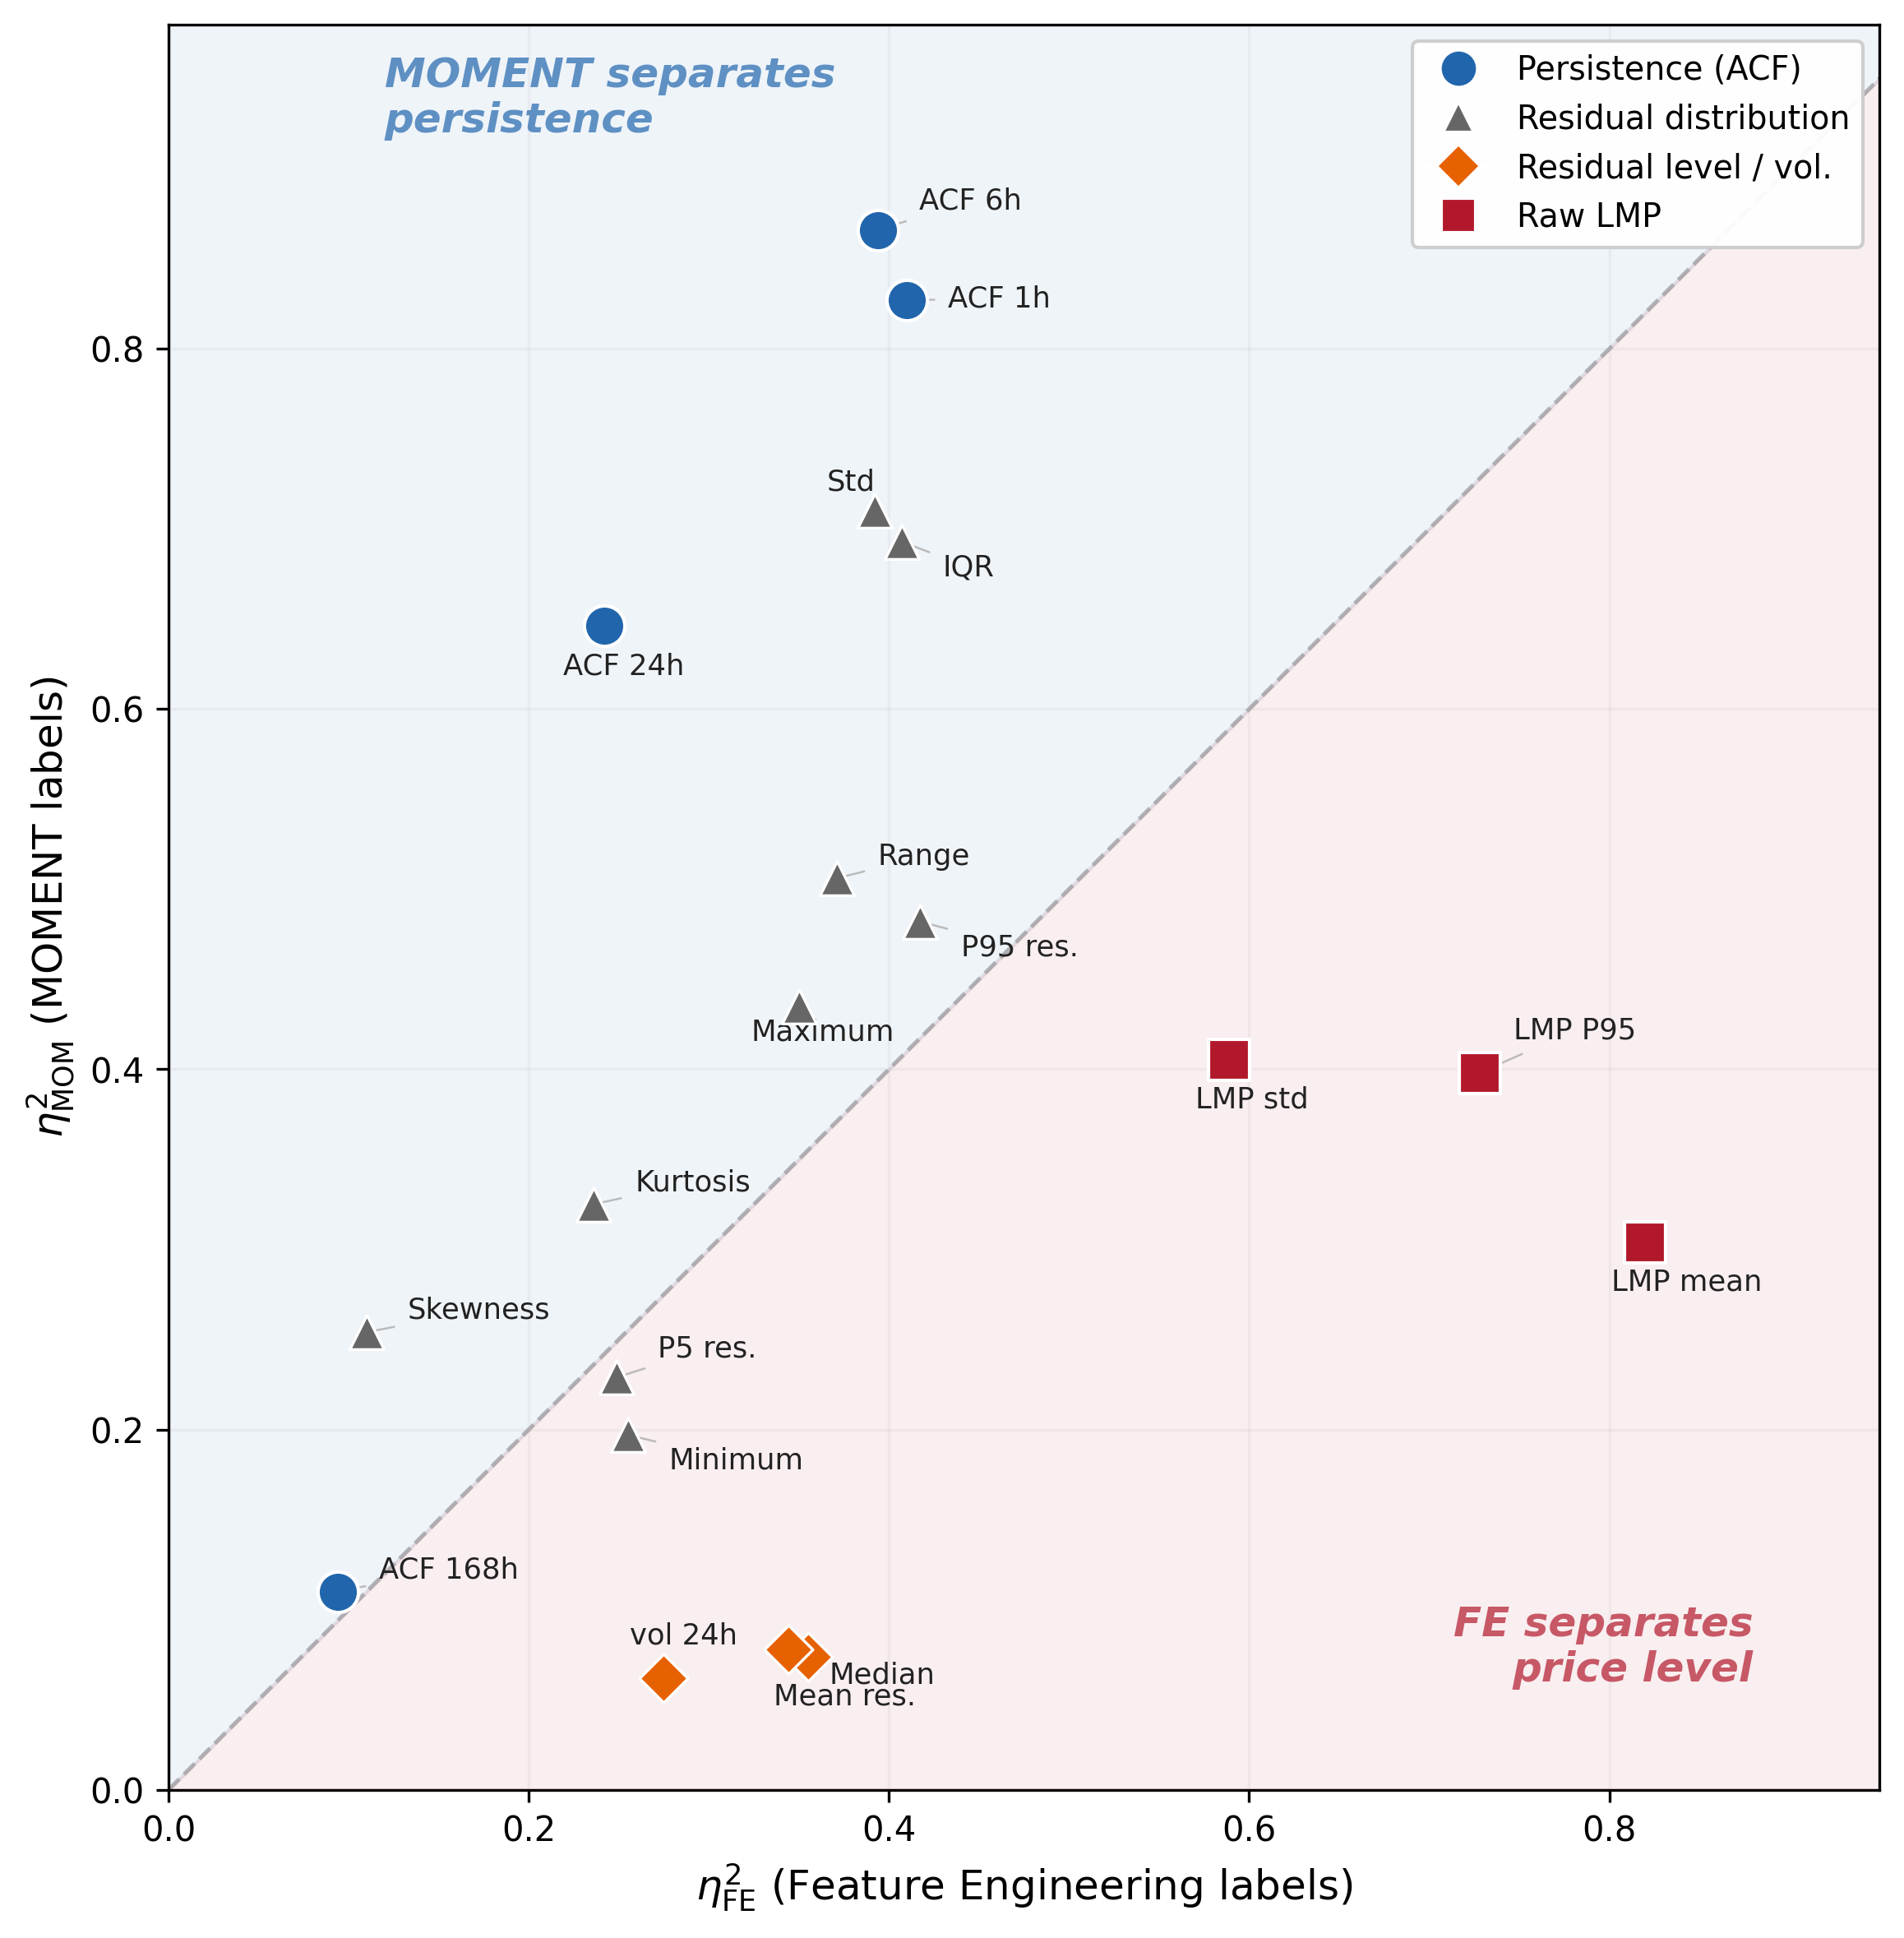
\includegraphics[width=0.78\textwidth]{cross_projection_explained.png}
\caption{Cross-projection of the 19 hand-crafted features onto both sets of cluster labels. Each point is one feature; its horizontal coordinate is $\eta^2_\text{FE}$ and its vertical coordinate is $\eta^2_\text{MOM}$. The diagonal marks equal separation. The blue region contains features separated more strongly by MOMENT (persistence); the red region contains features separated more strongly by FE (price level).}
\label{fig:cross_projection}
\end{figure}

Table~\ref{tab:cross_projection} reports the full cross-projection, sorted by the difference $\eta^2_\text{MOM} - \eta^2_\text{FE}$.
FE clusters explain up to 82\% of LMP variance but only 39\% of ACF variance; MOMENT clusters explain up to 87\% of ACF variance but only 30\% of LMP variance.

\begin{table}[H]
\centering
\caption{Cross-projection: $\eta^2$ of each feature with respect to FE and MOMENT cluster labels.}
\label{tab:cross_projection}
\small
\begin{tabular}{llcc}
\toprule
Feature & Captures & $\eta^2_\text{FE}$ & $\eta^2_\text{MOM}$ \\
\midrule
ACF lag 6\,h     & Intra-day persistence       & 0.394 & \textbf{0.866} \\
ACF lag 24\,h    & Residual diurnal persistence & 0.242 & \textbf{0.646} \\
ACF lag 1\,h     & Hour-to-hour persistence     & 0.410 & \textbf{0.827} \\
Std residual     & Volatility                   & 0.392 & \textbf{0.710} \\
IQR              & Robust dispersion            & 0.407 & \textbf{0.693} \\
Range            & Total excursion              & 0.371 & 0.506 \\
Kurtosis         & Tail heaviness               & 0.236 & 0.325 \\
Skewness         & Asymmetry                    & 0.110 & 0.254 \\
Maximum          & Peak value                   & 0.350 & 0.435 \\
$Q_{95}$ residual & Upper tail                  & 0.417 & 0.482 \\
ACF lag 168\,h   & Weekly persistence           & 0.094 & 0.110 \\
$Q_5$ residual   & Lower tail                   & 0.249 & 0.229 \\
Minimum          & Trough value                 & 0.255 & 0.197 \\
Mean residual    & Deseasonalized level         & 0.355 & 0.074 \\
vol\_24h         & Intra-day volatility         & 0.275 & 0.062 \\
Median           & Center                       & 0.344 & 0.078 \\
LMP $Q_{95}$     & Absolute spike level         & \textbf{0.728} & 0.398 \\
LMP std          & Absolute volatility          & \textbf{0.589} & 0.405 \\
LMP mean         & Absolute price level         & \textbf{0.820} & 0.304 \\
\bottomrule
\end{tabular}

\medskip
\small
\textit{Note}: Bold values indicate the dominant axis for that feature ($\eta^2 > 0.5$). Sorted by $\eta^2_\text{MOM} - \eta^2_\text{FE}$ (descending).
\end{table}

This cross-projection reveals two findings.
First, FE clusters separate price level (LMP mean: $\eta^2_\text{FE} = 0.82$), so the natural merge variable for FE is LMP.
Second, MOMENT clusters separate temporal persistence (ACF 6h: $\eta^2_\text{MOM} = 0.87$), so the natural merge variable for MOMENT is ACF at lag 6\,h.
The axis labels, ``economic'' for FE and ``dynamic'' for MOMENT, are assigned \emph{a posteriori} based on these results.


% ── 3.2 Economic Axis ────────────────────────────────────────────────────────
\subsection{Economic Axis}
\label{sec:economic_axis}

Since the cross-projection identifies mean LMP as the variable that FE separates most strongly, we merge the 35 initial FE modes by Tukey HSD on mean LMP ($\alpha = 0.05$).
Nine regimes survive, every pair significantly different in mean LMP.
For each window, define its average raw price as
\begin{equation}
\bar{p}_i =
\frac{1}{W}\sum_{h=0}^{W-1}p_{t_i-h}.
\label{eq:window_mean_lmp}
\end{equation}
The mean price of economic regime $k$ is then the average of $\bar{p}_i$ over the windows assigned to that regime:
\begin{equation}
\mu_k^{E}
=
\frac{1}{n_k^{E}}
\sum_{i:e_i=k}
\bar{p}_i.
\label{eq:economic_regime_mean}
\end{equation}
Ordering the regimes by $\mu_k^{E}$ gives the economic ladder in Table~\ref{tab:regimes}.
Figure~\ref{fig:merge_process} illustrates the merge: the 35 initial modes collapse into 9 regimes with a clean price gradient.

\begin{figure}[H]
\centering

\includegraphics[width=0.85\textwidth]{merge_process.png}
\caption{Tukey HSD merge on the economic axis. \textbf{Top}: 35 initial ToMATo modes, plotted by mean LMP. Many modes have nearly identical prices. \textbf{Bottom}: after iterative merging, 9 regimes survive, each significantly different from all others.}
\label{fig:merge_process}
\end{figure}

\begin{table}[H]
\centering
\caption{Characterization of 9 economic regimes, ordered by mean LMP.}
\label{tab:regimes}
\small
\setlength{\tabcolsep}{4pt}
\begin{tabular}{clrrrcl}
\toprule
ID & LMP $\mu$ & LMP $\sigma$ & $n$ & \% & Dominant season & Interpretation \\
\midrule
R5 & 27.5  & 9.0  & 821  & 11.4 & Spring (30\%)    & Off-peak \\
R3 & 33.3  & 16.2 & 701  & 9.7  & Autumn (38\%)    & Low \\
R1 & 39.3  & 26.0 & 1,621 & 22.5 & Autumn (35\%)   & Below-average \\
R0 & 46.2  & 20.2 & 1,272 & 17.6 & Autumn (39\%)   & Baseload \\
R2 & 57.1  & 35.8 & 532  & 7.4  & Winter (47\%)    & Moderate \\
R4 & 72.0  & 40.0 & 1,024 & 14.2 & Winter (34\%)   & Demand \\
R6 & 80.4  & 48.1 & 435  & 6.0  & Winter (38\%)    & Stress \\
R7 & 92.2  & 53.2 & 385  & 5.3  & Winter (65\%)    & Winter spike \\
R8 & 137.2 & 50.7 & 426  & 5.9  & Winter (94\%)    & Extreme spike \\
\bottomrule
\end{tabular}

\medskip
\small
\textit{Note}: $n$ = number of windows assigned to regime. \% = share of total windows. Dominant season = season with highest share of windows.
\end{table}

The 9 regimes span \$27.5--137.2/MWh with monotonically increasing mean and volatility.
Low-price regimes concentrate in spring/autumn; high-price regimes in winter, reflecting New England's gas-dependency for heating \citep{isone2024}.

Temporal coherence is excellent.
The transition rate, computed as
\begin{equation}
\pi_E =
\frac{1}{N-1}
\sum_{i=1}^{N-1}
\mathbf{1}\{e_{i+1}\neq e_i\},
\label{eq:transition_rate}
\end{equation}
is only 2.9\% at 6-hour resolution.
The sojourn time is computed by grouping consecutive windows with the same label into runs.
A run of $m$ consecutive windows in regime $k$ corresponds to a sojourn of
\begin{equation}
\tau = m \cdot S
\label{eq:sojourn}
\end{equation}
hours, where $S=6$ is the stride.
The mean sojourn time across all runs is 205 hours ($\approx$8.5 days), consistent with the physical time scales of weather systems and fuel-market dynamics.
Transitions occur predominantly between adjacent price levels: R8 moves only to R6 or R7, never directly to low-price regimes.
R8 has the longest sojourn (511 hours, $\approx$21 days), consistent with the sustained nature of winter cold events.
Descriptively, the 9 regimes account for 42.5\% of LMP variance ($\eta^2 = 0.425$).


% ── 3.3 Dynamic Axis ─────────────────────────────────────────────────────────
\subsection{Dynamic Axis}
\label{sec:dynamic_axis}

Since the cross-projection identifies ACF at lag 6\,h as the variable that MOMENT separates most strongly, we merge the 68 initial MOMENT modes by Tukey HSD on ACF at lag 6\,h (Figure~\ref{fig:merge_dynamic}).
Eight regimes survive, every pair significantly different in ACF at lag 6\,h.
These regimes switch faster than the economic axis (20\% transition rate, mean sojourn 30\,h) but are temporally coherent at the sub-daily scale.

\begin{figure}[H]
\centering

\includegraphics[width=0.85\textwidth]{merge_process_dynamic.png}
\caption{Tukey HSD merge illustrated on the dynamic axis. \textbf{Top}: 68 initial ToMATo modes, plotted by mean ACF at lag 6\,h. Many modes have nearly identical persistence. \textbf{Bottom}: after iterative merging, 8 regimes survive, each significantly different from all others.}
\label{fig:merge_dynamic}
\end{figure}

Table~\ref{tab:dynamic_regimes} presents the 8 dynamic regimes, ordered by mean ACF at lag 6\,h.
For a window $i$, the lag-6 autocorrelation is computed on the $W=512$ residual values in $\mathbf{r}_i$.
Let $r_{i,h}$ denote the $h$-th hourly residual inside window $i$ (with $h=1,\ldots,W$) and $\bar{r}_i = \frac{1}{W}\sum_{h=1}^{W} r_{i,h}$ the window mean.
The sample autocorrelation at lag 6 is
\begin{equation}
\widehat{\rho}_{6,i}
=
\frac{\sum_{h=7}^{W}
(r_{i,h}-\bar{r}_i)(r_{i,h-6}-\bar{r}_i)}
{\sum_{h=1}^{W}(r_{i,h}-\bar{r}_i)^2},
\label{eq:window_acf6}
\end{equation}
where the numerator sums over the $W-6$ pairs of observations separated by 6 hours and the denominator is the total sum of squares of the window.
The mean persistence of dynamic regime $\ell$ is
\begin{equation}
\mu_\ell^{D}
=
\frac{1}{n_\ell^{D}}
\sum_{i:d_i=\ell}
\widehat{\rho}_{6,i}.
\label{eq:dynamic_regime_mean}
\end{equation}
The regimes span a wide range: from D0 ($\mu^D = 0.32$, shocks dissipate within hours) to D7 ($\mu^D = 0.88$, shocks persist for days).
Crucially, price level is not monotonic across dynamic regimes: D4 (ACF $= 0.76$, summer) has a lower mean LMP (\$48.6/MWh) than D3 (ACF $= 0.68$, winter, \$59.2/MWh), confirming that the dynamic axis captures a dimension genuinely independent of price.

\begin{table}[H]
\centering
\caption{Characterization of 8 dynamic regimes, ordered by mean ACF at lag 6\,h.}
\label{tab:dynamic_regimes}
\small
\setlength{\tabcolsep}{4pt}
\begin{tabular}{clrrrrcl}
\toprule
ID & ACF$_\text{6h}$ $\mu$ & $\sigma_r$ & LMP $\mu$ & $n$ & \% & Dominant season & Interpretation \\
\midrule
D0 & 0.316 & 0.131 & 37.9 & 1{,}202 & 16.7 & Spr/Aut          & Fast-reverting \\
D1 & 0.521 & 0.148 & 47.8 & 2{,}094 & 29.0 & Autumn (42\%)    & Normal \\
D2 & 0.651 & 0.223 & 52.1 & 629     & 8.7  & Summer (91\%)    & Summer-persistent \\
D3 & 0.684 & 0.184 & 59.2 & 471     & 6.5  & Winter (45\%)    & Moderate \\
D4 & 0.759 & 0.242 & 48.6 & 749     & 10.4 & Summer (75\%)    & Summer-sticky \\
D5 & 0.780 & 0.240 & 61.8 & 659     & 9.1  & Winter (56\%)    & Winter-sticky \\
D6 & 0.837 & 0.328 & 79.3 & 310     & 4.3  & Winter (63\%)    & Stress-persistent \\
D7 & 0.883 & 0.384 & 84.7 & 1{,}103 & 15.3 & Winter (72\%)    & Shock-persistent \\
\bottomrule
\end{tabular}

\medskip
\small
\textit{Note}: $\sigma_r$ = mean standard deviation of the MSTL residual within the window. LMP $\mu$ in \$/MWh.
\end{table}

Three patterns merit discussion.
First, persistence is not exclusively a winter phenomenon: D2 and D4 are summer-dominated regimes with ACF above 0.65, driven by sustained air-conditioning demand during heat waves.
The dynamic axis distinguishes two distinct summer dynamics, moderately persistent (D2) and sticky (D4), that a single ``summer'' label would conflate.
Second, D7 is the second-largest high-persistence regime (15.3\% of windows, mean sojourn 95\,h $\approx$ 4 days), indicating that shock-persistent market states are not rare tail events but a substantial fraction of market time.
Third, volatility ($\sigma_r$) increases monotonically with persistence: fast-reverting markets are calm ($\sigma_r = 0.13$), shock-persistent markets are turbulent ($\sigma_r = 0.38$).
This persistence--volatility coupling is consistent with volatility clustering in financial markets but here it is captured as a structural regime property rather than an autoregressive effect.


% ── 5.3 Two-Axis Structure ───────────────────────────────────────────────────
\subsection{Two-Axis Structure}
\label{sec:two_axes}

The previous two sections have shown that the economic axis separates price levels and the dynamic axis separates temporal persistence.
But are these two views of the same underlying structure, or do they capture genuinely different dimensions?
If the two partitions largely agree, then one axis is redundant and a single regime label suffices.
If they disagree, the market state requires two labels: one for price level and one for persistence.

To quantify the overlap between the two partitions, we use the Adjusted Rand Index (ARI).
The ARI considers every pair of windows and checks whether the two partitions agree on them: do both place the pair in the same group, or do both place them in different groups?
The index counts how many pairs agree, corrects for the agreement expected by chance, and normalizes the result so that its expected value under random labeling is 0 and perfect agreement gives 1.

The computation starts from the contingency table between the two partitions.
Let $n_{ij}$ be the number of windows assigned to economic regime $i$ and dynamic regime $j$, and let $a_i = \sum_j n_{ij}$ and $b_j = \sum_i n_{ij}$ be the row and column totals.
The ARI is then
\begin{equation}
\text{ARI} = \frac{\sum_{ij}\binom{n_{ij}}{2} - \left[\sum_i\binom{a_i}{2}\sum_j\binom{b_j}{2}\right]\!/\!\binom{n}{2}}{\frac{1}{2}\!\left[\sum_i\binom{a_i}{2}+\sum_j\binom{b_j}{2}\right] - \left[\sum_i\binom{a_i}{2}\sum_j\binom{b_j}{2}\right]\!/\!\binom{n}{2}}.
\label{eq:ari}
\end{equation}
The numerator counts pair agreements beyond chance; the denominator normalizes by the maximum possible excess.

The ARI between the economic and dynamic partitions is \textbf{0.09}, very close to zero and far below the threshold of 0.5 typically considered indicative of meaningful agreement.
This means that knowing a window's economic regime tells us almost nothing about its dynamic regime, and vice versa.
The two axes are \emph{nearly orthogonal}: they organize the same windows in fundamentally different ways.
The evidence for this orthogonality rests on three independent lines.

First, the ARI value itself: 0.09 means the two partitions share only marginally more structure than two random labelings would.

Second, Figure~\ref{fig:axes_evidence} shows that each axis cleanly separates what the other cannot.
The figure has four panels arranged as a $2\times 2$ cross-pattern:
\begin{itemize}[nosep]
\item[\textbf{(a)}] FE regimes vs.\ LMP: a clean monotonic staircase; each regime occupies a distinct price band. FE separates price level.
\item[\textbf{(b)}] MOMENT regimes vs.\ LMP: heavily overlapping distributions, no price gradient. MOMENT does \emph{not} separate price level.
\item[\textbf{(c)}] MOMENT regimes vs.\ ACF at lag 6\,h: a clean monotonic gradient from fast-reverting to sticky. MOMENT separates temporal persistence.
\item[\textbf{(d)}] FE regimes vs.\ ACF at lag 6\,h: flat, overlapping distributions. FE does \emph{not} separate persistence.
\end{itemize}
The cross-pattern --- panels (a) and (c) show separation while (b) and (d) do not --- is the visual fingerprint of orthogonality: each representation captures a dimension that the other largely misses.

\begin{figure}[H]
\centering
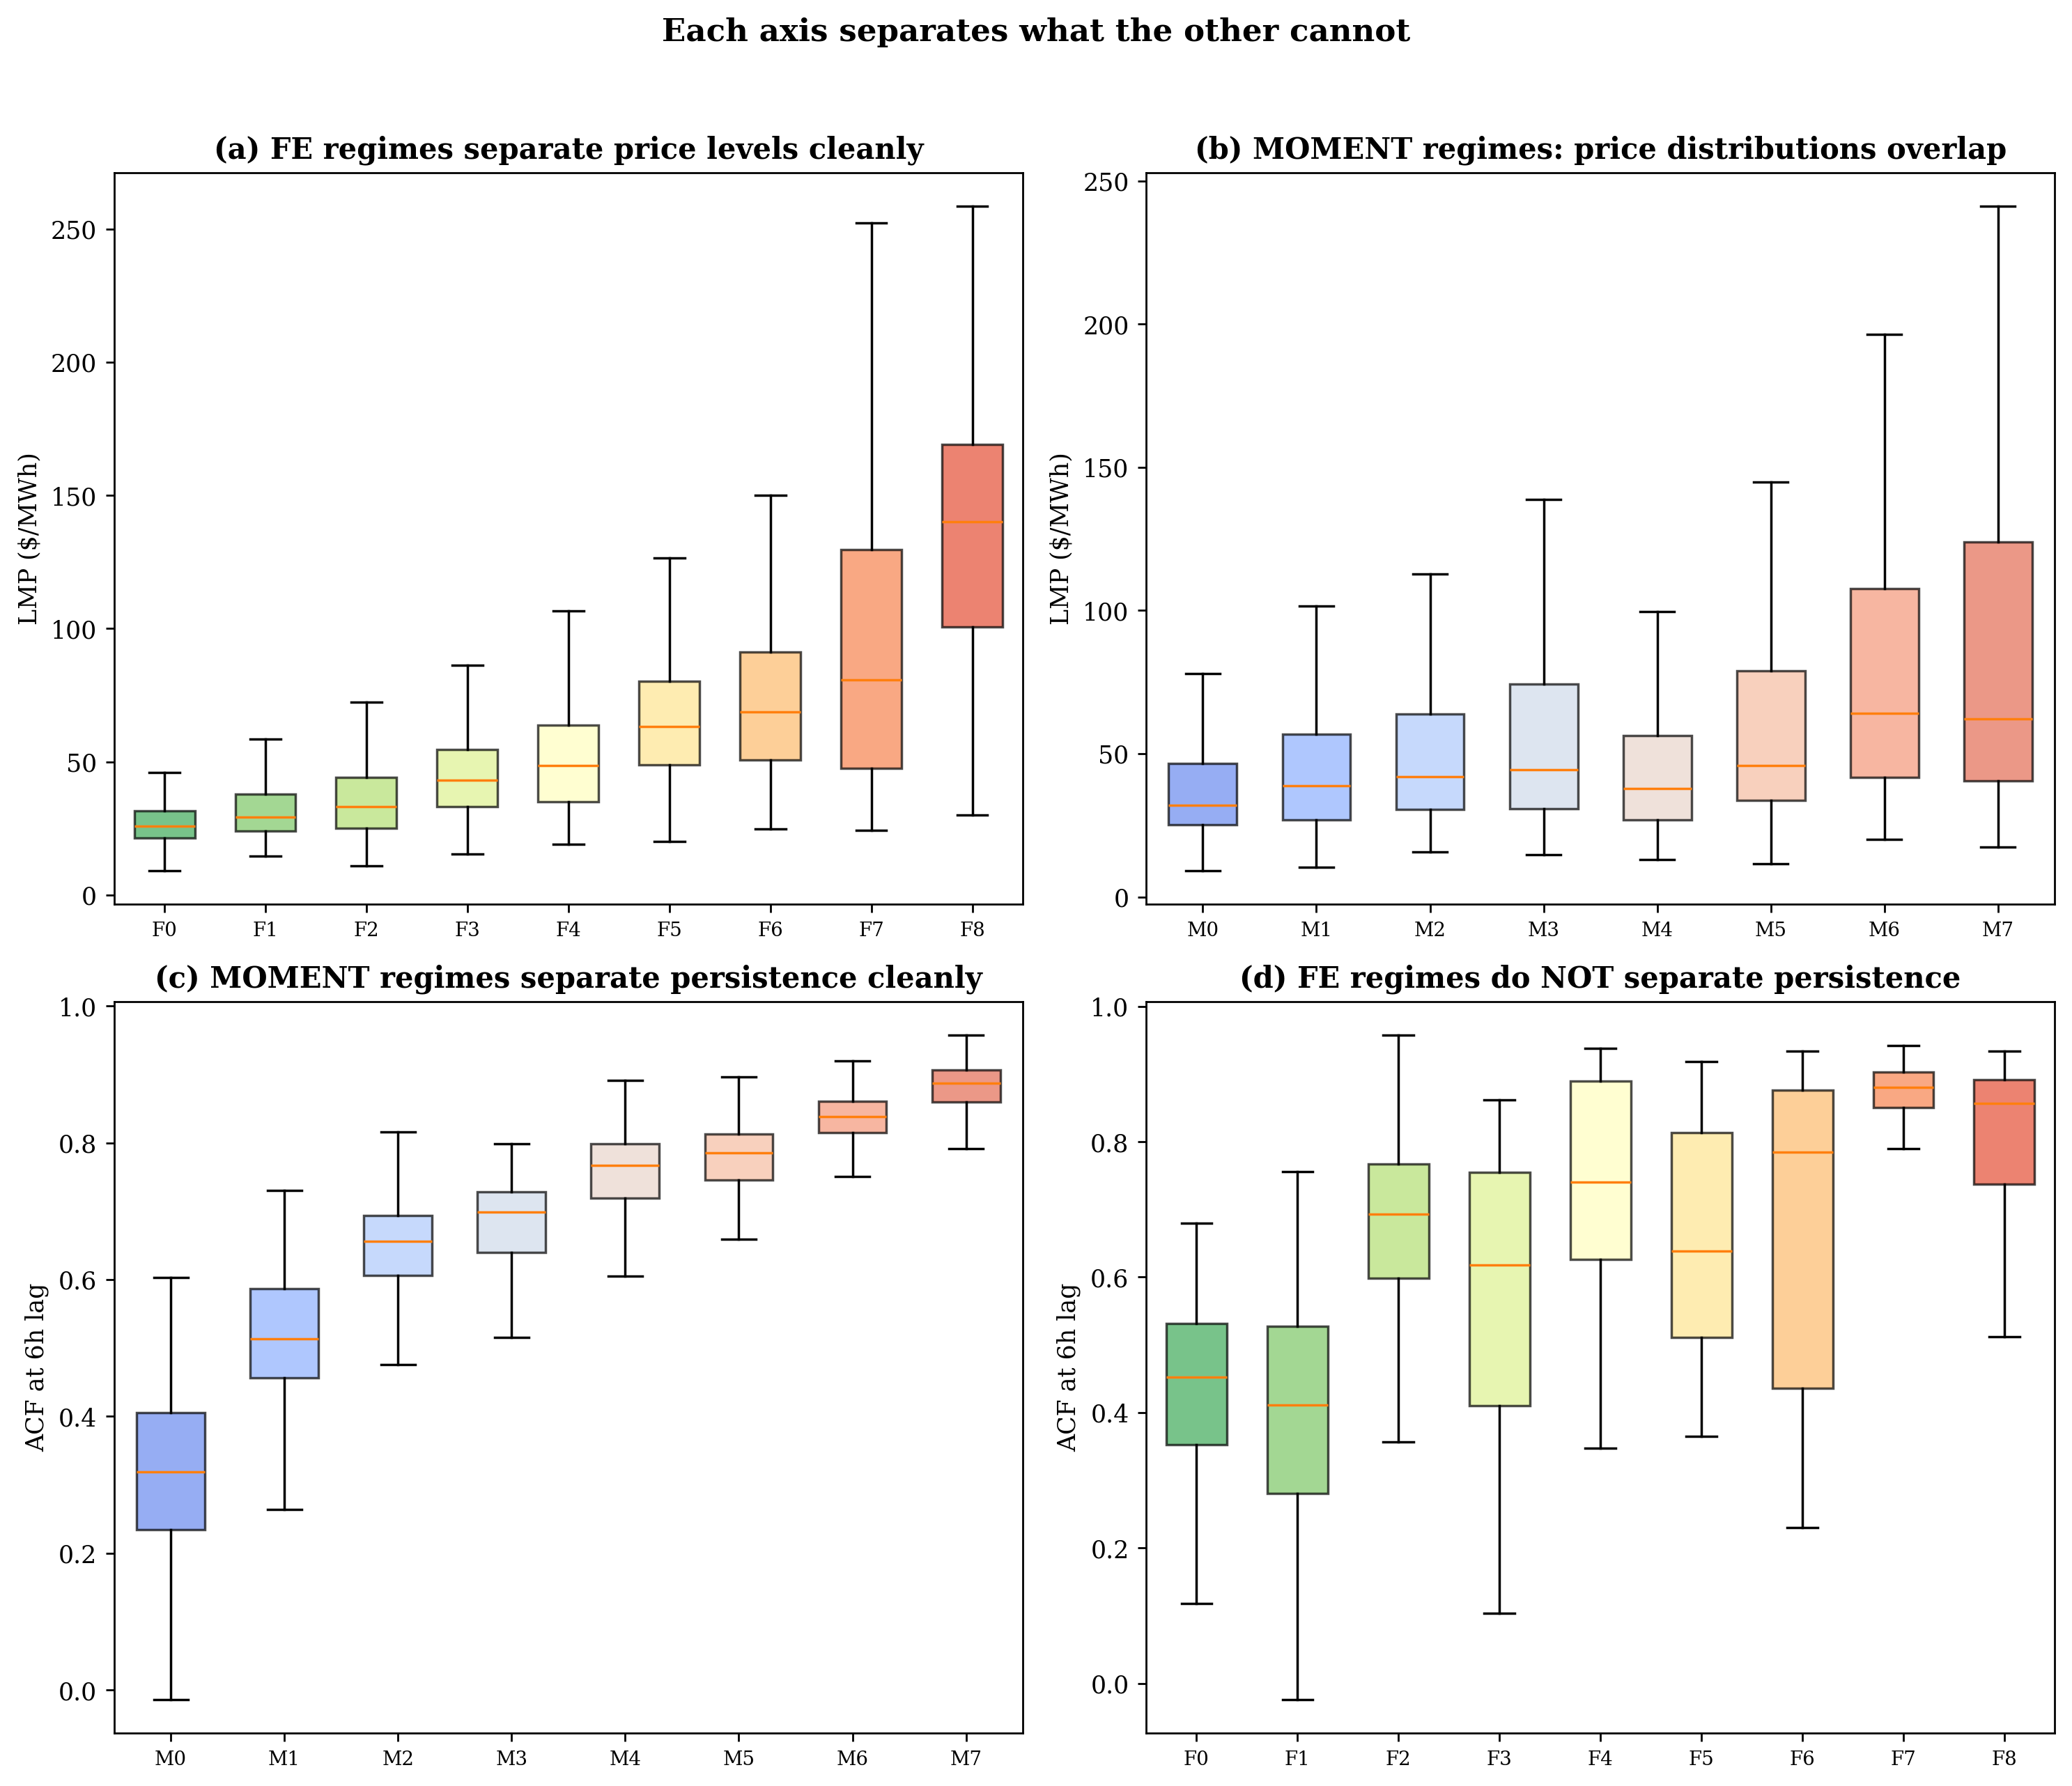
\includegraphics[width=\textwidth]{axes_evidence.png}
\caption{Each axis separates what the other cannot. \textbf{(a)}~FE regimes produce a monotonic price gradient. \textbf{(b)}~MOMENT regimes do not separate price. \textbf{(c)}~MOMENT regimes produce a monotonic persistence gradient. \textbf{(d)}~FE regimes do not separate persistence.}
\label{fig:axes_evidence}
\end{figure}

Third, all four combinations of high/low price and high/low persistence are populated (Figure~\ref{fig:two_axes}).
If the two axes were redundant, some combinations would be empty --- for example, high-price markets would always be sticky, or low-price markets would always revert quickly.
Instead, every quadrant contains a substantial fraction of the data.

To construct this view, we reduce the two ordered label vectors to a binary summary.
Let $c_E$ be the median of the economic regime means $\{\mu_k^E\}$ and $c_D$ the median of the dynamic regime means $\{\mu_\ell^D\}$, so that the cut falls between the two middle regimes on each axis.
For each window,
\begin{equation}
H_i=\mathbf{1}\{\mu_{e_i}^{E}>c_E\},
\qquad
S_i=\mathbf{1}\{\mu_{d_i}^{D}>c_D\}.
\label{eq:quadrant_indicators}
\end{equation}
The four resulting quadrants each correspond to a distinct market state:
\begin{itemize}[nosep]
\item \textbf{Low price, fast-reverting} (34\%): calm conditions in mild weather. Normal operations suffice; hedging exposure is low.
\item \textbf{Low price, sticky} (38\%): prolonged moderate or low-price periods. Renewable curtailment risk is elevated; storage operators have an incentive to charge.
\item \textbf{High price, fast-reverting} (8\%): transient spikes that resolve within hours. Aggressive hedging in this state may be unnecessarily costly.
\item \textbf{High price, sticky} (20\%): sustained stress events, typically winter cold snaps. Hedging is warranted; emergency reserves may be depleted over days.
\end{itemize}
No single-axis partition can distinguish these four states.
In particular, the conventional ``spike'' label lumps transient and persistent high-price events, even though their risk profiles are qualitatively different: the first resolves on its own, the second requires active intervention.

\begin{figure}[H]
\centering

\includegraphics[width=0.72\textwidth]{two_axis_grid.png}
\caption{Dual-axis regime space. Each quadrant represents a distinct market state. All four quadrants are populated, confirming that price level and persistence vary independently.}
\label{fig:two_axes}
\end{figure}


% ══════════════════════════════════════════════════════════════════════════════
\section{Discussion}
\label{sec:discussion}

Table~\ref{tab:comparison} summarizes the two axes before discussing their implications.

\begin{table}[H]
\centering
\caption{Characterization of the two axes.}
\label{tab:comparison}
\small
\begin{tabular}{lccccc}
\toprule
Axis & & $\eta^2$ & Trans\% & Sojourn & Tukey \\
\midrule
Economic (FE)   & $K_E = 9$ & 0.425$^\text{LMP}$  & 2.9\%  & 205\,h & 36/36 \\
Dynamic (MOMENT) & $K_D = 8$ & 0.866$^\text{ACF}$  & 20.0\% & 30\,h  & 28/28 \\
\bottomrule
\end{tabular}

\medskip
\small
\textit{Note}: $\eta^2$ is reported on each axis's primary target variable (LMP for economic, ACF at lag 6\,h for dynamic).
Trans\% = transition rate at 6-hour resolution; Sojourn = mean sojourn time; Tukey = significant pairs / total pairs ($\alpha = 0.05$) on the primary target.
\end{table}

The two axes have direct practical consequences.
The economic axis answers \emph{how much} electricity costs; the dynamic axis answers \emph{how} the price will behave over the next hours and days.
All four combinations of high/low price and fast/slow mean-reversion are populated (Figure~\ref{fig:two_axes}), each with distinct operational meaning.
High-price, fast-reverting states (8\% of windows) are transient spikes that resolve quickly, aggressive hedging would over-pay.
High-price, shock-persistent states (20\%) are sustained stress events, typically winter cold snaps, where hedging is warranted and emergency reserves may be depleted.
Low-price, fast-reverting states (34\%) are calm markets in mild weather where normal operations suffice.
Low-price, sticky states (38\%) are prolonged periods of moderate or low prices where renewable curtailment risk is elevated and storage operators should charge.
A conventional single-axis ``spike'' label lumps transient and persistent high-price events, even though their risk profiles are qualitatively different.

% --- Why MOMENT captures dynamics ---

An important question is \emph{why} MOMENT separates temporal persistence while hand-crafted features do not, despite the FE representation containing explicit ACF features.
The answer lies in the dimensionality balance: the 4 ACF features comprise 21\% of the 19-dimensional FE space, but the remaining 15 distributional and price-level features dominate the manifold geometry in Diffusion Maps.
MOMENT, by contrast, receives only the raw 512-hour residual and encodes temporal structure as its \emph{primary} signal: its masked-reconstruction pre-training objective forces the encoder to learn how patterns evolve over time, precisely the information that ACF measures.
The 1,024-dimensional MOMENT embedding collapses to just 2 diffusion coordinates, suggesting that the foundation model's internal representation is organized along a small number of dominant temporal modes.

% --- Relation to existing literature ---

The two-axis structure connects to the regime-switching literature in a novel way.
Classical HMM approaches assume a single latent state that drives both the price level and the volatility dynamics simultaneously.
Our finding suggests that this assumption may be too restrictive: level and persistence appear to be governed by independent latent processes.
A market can be in a high-price economic regime and a fast-reverting dynamic regime simultaneously, a combination that a single-chain HMM cannot represent without an exponential expansion of the state space.

% --- Validation framework ---

The validation framework is deliberately multi-dimensional: Tukey HSD ensures statistical distinctness within each axis, and temporal coherence (sojourn times, adjacent-only transitions) confirms that the regimes reflect physical market dynamics rather than statistical artifacts.
No single scalar metric can adequately compare a partition that separates price levels against one that separates temporal dynamics; the cross-projection analysis (Table~\ref{tab:cross_projection}) and the near-zero ARI together establish that the two axes capture genuinely different aspects of market structure.

% --- Why price-only ---

The pipeline deliberately operates on price data alone.
In competitive wholesale markets, the LMP already aggregates supply-side and demand-side information via the merit-order dispatch: a spike in gas prices, a wind drought, or a generator outage all manifest in the LMP before they appear in any exogenous variable.
Exogenous variables (temperature, gas spot prices, renewable forecast errors) could reveal further orthogonal dimensions, and the cross-ARI framework provides the tool to test this: any new representation that produces a partition with near-zero ARI against both known axes would constitute a genuine third dimension of market structure.

% --- Limitations ---

Several limitations should be acknowledged.
The overlapping sliding windows ($S/W = 6/512$) inflate the nominal sample size; the effective number of independent 21-day windows is approximately 85.
The 9-regime economic partition represents a fine-grained slicing of a continuous price gradient; the number of distinguishable regimes depends on statistical power, but the monotonic gradient and all-pairs significance are preserved.
The analysis covers a single market (ISONE) and pricing node; generalization to other ISOs requires further study.
The foundation model is applied zero-shot; domain-specific fine-tuning might strengthen the dynamic axis.
The 512-hour window imposes a minimum time scale, and the pipeline is retrospective; real-time regime forecasting remains future work.

% ══════════════════════════════════════════════════════════════════════════════
\section{Conclusion}
\label{sec:conclusion}

This paper introduces a non-parametric pipeline for unsupervised regime detection in electricity spot markets, in which the number of regimes, the manifold dimensionality, and all tuning parameters emerge from the data through topological persistence analysis.
Applying this pipeline to five years of ISO New England hourly prices with two alternative representations, we arrive at a structural finding: the electricity market is organized along at least two independent axes of regime structure.

The first axis is economic: 19 domain-specific features yield $K_E = 9$ regimes spanning off-peak to extreme winter spike.
These regimes persist for days and transition gradually through adjacent price levels.

The second axis is dynamic: MOMENT yields $K_D = 8$ regimes, separated by temporal persistence and volatility, how quickly the market mean-reverts after a shock.
$K_E$ and $K_D$ differ because each axis partitions a different dimension of the data; both emerge from the same pipeline without analyst intervention.
The two axes are statistically independent.

No single representation suffices: economic regimes serve hedging, dynamic regimes serve forecasting, and the two must be deployed in parallel.

The pipeline (Diffusion Maps, ToMATo, and Tukey HSD merging) provides a principled, reproducible methodology that requires no prior assumption on the number of market states and can be directly transferred to other markets and commodity price series.
The cross-ARI framework introduced here also provides a tool for future work: any new representation (frequency-domain features, multivariate embeddings, exogenous variables) that produces a partition with near-zero ARI against both known axes would constitute a genuine addition to the dimensionality of market structure.

% ══════════════════════════════════════════════════════════════════════════════
\bibliographystyle{plainnat}
\bibliography{references}

\end{document}
